\documentclass[12pt]{report}
\usepackage[utf8]{inputenc}
\usepackage{amsmath, amssymb}
\usepackage{graphicx}
\usepackage{geometry}
\usepackage{float}
\usepackage{color}
\usepackage{caption}
\usepackage{listings} % for code snippets
\usepackage{xcolor} % for customizing colors
\usepackage{amssymb}
\usepackage{minted}
\usepackage{rotating}
\usepackage{hyperref}
\usepackage{cite}
\usepackage{algorithm}
\usepackage{algpseudocode}
\usepackage{subcaption}
\usepackage{booktabs}
\usepackage{packages/kbordermatrix}
\usepackage{packages/slashbox}
\usepackage{diagbox}
\geometry{a4paper, total={170mm,257mm},left=15mm, right=15mm, top=20mm}
\graphicspath{ {media/} }
\setcounter{secnumdepth}{3}


\geometry{margin=1in}

\definecolor{codegray}{gray}{0.95}
\lstset{
  backgroundcolor=\color{codegray},
  basicstyle=\ttfamily\small,
  breaklines=true,
  postbreak=\mbox{\textcolor{red}{$\hookrightarrow$}\space},
  frame=single
}

\lstset{
    language=Matlab,            % Set the language to Matlab
    basicstyle=\ttfamily\small, % Set font and size
    keywordstyle=\color{blue},  % Keywords in blue
    stringstyle=\color{green},  % Strings in green
    commentstyle=\color{gray},  % Comments in gray
    showstringspaces=false,     % Do not display spaces in strings
    numbers=left,               % Line numbers on the left
    numberstyle=\tiny\color{gray}, % Style for line numbers
    frame=single,               % Add a frame around the code
    breaklines=true,            % Allow line breaking
    captionpos=b,               % Caption at the bottom
}


\begin{document}
\begin{titlepage}
\begin{center}
    \vspace{1cm}

    \begin{figure}[h]
        \centering
        \includegraphics[width=8cm]{AUTH_Banner.png}
    \end{figure}
    
    \vspace{2cm}
    \Huge\textbf{Analysis of Axelrod Tournament Meetings and Methodology}\\
    \vspace{2.5cm}

    \Large\textbf{Group 03}
    \vspace{2.5cm}

        
    \Large\textbf{Collaborators}\\  
    \vspace{0.2cm}
    \large
    Kostantinos Fotis Papadakis, kpapadak@ece.auth.gr\\ 
    \vspace{0.2cm}
    Grigoris Daios, grigorad@ece.auth.gr \\  
    \vspace{0.2cm}
    Ioannis Georgiou Mousses, georgioui@ece.auth.gr  \\  
    \vspace{0.2cm}
    Sokratis Nazlidis, snazlidi@ece.auth.gr \\  
    \vspace{2cm}
    
    
\begin{center}
        \large{\textbf{Department of Electrical and \\ Computer Engineering, AUTH}}\\ May 2025
        
    \end{center}
\end{center}
\end{titlepage}

\tableofcontents
\newpage
\chapter{Introduction}
\section{The problem at hand}
In the following report, we examine the dynamics of \textbf{evolutionary games}-games played over successive generations in large populations. These games consist of:
\begin{itemize}
    \item A \textbf{base game}, such as the Iterated Prisoner's Dilemma.
    \item A \textbf{population} of players.
    \item A \textbf{pool of strategies} available to players.
    \item A \textbf{match}, defined as a play between two players.
    \item A \textbf{meeting}, which includes all possible matches in the population.
\end{itemize}
The evolutionary game progresses through a sequence of meetings, with each new generation adopting strategies based on performance. Initially, strategy adoption is random, but over time, better-performing strategies prevail. While some games converge to a single dominant strategy, others exhibit \textbf{oscillations}, \textbf{sensitivity to initial conditions}, or even \textbf{chaotic patterns}.
This report focuses on two mechanisms that drive these evolutionary changes:
\begin{itemize}
    \item \textbf{Imitation dynamics}-players mimic successful strategies from the previous generation.
    \item \textbf{Fitness dynamics}-strategies spread in proportion to their payoff.
\end{itemize}
Through the above models, we explore how strategy performance shapes long-term behavior in populations. It is ultimately revealed that cooperation is not always the inevitable outcome.
\section{Related work}
This report builds on earlier work by Axelrod and Hamilton (1981) \cite{axelrod1981}, Axelrod and Dion (1988) \cite{axelrod1988}, and the book "Evolutionary Game Theory
" by J. McKenzie Alexander (2023) \cite{alexander2023}.
Furthermore,“Studies on Dynamics in the
Classical Iterated Prisoner’s Dilemma with Few Strategies” by Mathieu,  Beaufils and  Delahaye (1999) \cite{mathieu1999} questions the assumption that cooperation always dominates,by presenting other complex dynamics and highlighting the role of initial conditions in final simulation outcomes.\\
For the Markov Theory part, we based our work on: “The Iterated Prisoner's Dilemma” \cite{wolfram}, “Zero-Determinant Strategies in the Iterated Prisoner's Dilemma” \cite{ncategory} and “Iterated Prisoner’s Dilemma contains strategies that dominate any evolutionary opponent” \cite{pressdyson2012}.


\section{Quick start-Brief intro to our code}
First and foremost, one can review our entire implementation here:\\ \url{https://github.com/Kou-ding/Prisoner-s-Dilemma}\\
Detailed presentation of the most important parts of the code can be found in the Appendix of this report.\\
Our entire \textbf{MATLAB toolbox} is based upon two sections:
\begin{itemize}
    \item \textbf{Genaxel}: Here we simulate and analyze strategy evolution within the Axelrod tournament. The implementation facilitates dIfferent modes of
fitness calculation and evolutionary dynamics.It also supports multiple tournament styles and population update mechanisms.
    \item  \textbf{Markov}: This second part of the project was implemented in a completely dIfferent way. Object-oriented programming was not the basis here. The logic is implementing 1 on 1 tournaments of 3 players, where populations change on the basis of implemented rules and States.
\end{itemize}
\subsection{How to run the project}
\begin{enumerate}
    \item Download the project locally
    \item navigate to \texttt{Examples/} directory
    \item Configure the \texttt{script.m} file to reflect the parameters you want to use
    \begin{itemize}
        \item Set \texttt{custom = true} to manually configure all parameters.
        \item Or set \texttt{custom = false} and load one of the pre-made meetings by uncommenting the corresponding \texttt{.fig} file under the \textbf{"Load your desired meeting"} section.
    \end{itemize}
\end{enumerate}
\subsection{Project directory overview}
\begin{tabular}{@{}ll@{}}
\toprule
\textbf{Folder / File} & \textbf{Description} \\
\midrule
\texttt{Code/Genaxel/} & Genetic Axelrod tournament (OOP) \\
\texttt{Code/Markov/} & Markov-related modules \\
\quad \texttt{Markov Theory/} & Theory documentation \\
\quad \texttt{Markov Simulation/} & Simulation setup and code \\
\texttt{Documentation/} & Function-level code documentation \\
\texttt{Examples/} & Demos and \texttt{script.m} setup \\
\texttt{Report/} & Final report PDF and LaTeX source \\
\bottomrule
\end{tabular}
\newpage
\section{Markov theory: Quick start}
\subsection{How to run}
All the files required are inside the Markov directory. In function \mintinline{matlab}{initialize()} we can choose the total population $N$, the payoff matrix (R, S, T, P), the rounds per match for the theoretical (\mintinline{matlab}{roundsth}) and the simulation (\mintinline{matlab}{roundssim}) parts, the number of repetitions per initial state \mintinline{matlab}{numofrep}, the number of generations \mintinline{matlab}{ngens} needed for the simulation part and the vector \mintinline{matlab}{chosen} of the three strategies to compete. If the calculations are to be based on the expected average payoff per round, the value of the variable \mintinline{matlab}{predetermined} should be set to the empty string ' '. If exact calculations based on the evaluation of the score as a deterministic function of the game history are to be used, we can choose the competitors by setting an appropriate string value for \mintinline{matlab}{predetermined} (see \mintinline{matlab}{initialize()} for details). After the theoretical calculations are performed and the respective graphs drawn, the user is asked if he wishes to continue with the simulation part (may be time demanding). There is no simulation part if predetermined outcome meetings are used. Run the script \mintinline{matlab}{MarkovRun.m}.

\subsection{How to add a new strategy with its strategy vector $\mathbf{p}$}

In \mintinline{matlab}{initialize()}, add the strategy's index and name in the map \mintinline{matlab}{names}, its name and strategy vector in map \mintinline{matlab}{ps} and its name and probability for the initial move to be C, in the map \mintinline{matlab}{pinitC}.

\subsection{How to add a new predetermined outcome meeting}

Use a new letter as a possible value of \mintinline{matlab}{predetermined} and add a new information message in the appropriate \mintinline{bash}{switch-case} in \mintinline{matlab}{initialize()}. Describe the calculation of the payoffs in a match between any two players, in the \mintinline{bash}{switch-case} of the function \mintinline{matlab}{deterministicPayoffs()}.

\clearpage
\subsection{Structure of matrix \mintinline{matlab}{allstaterepgenNumOfPlayersHistory} and plotting of the time evolution of the population of each strategy}

\begin{figure}[h!]
    \centering
    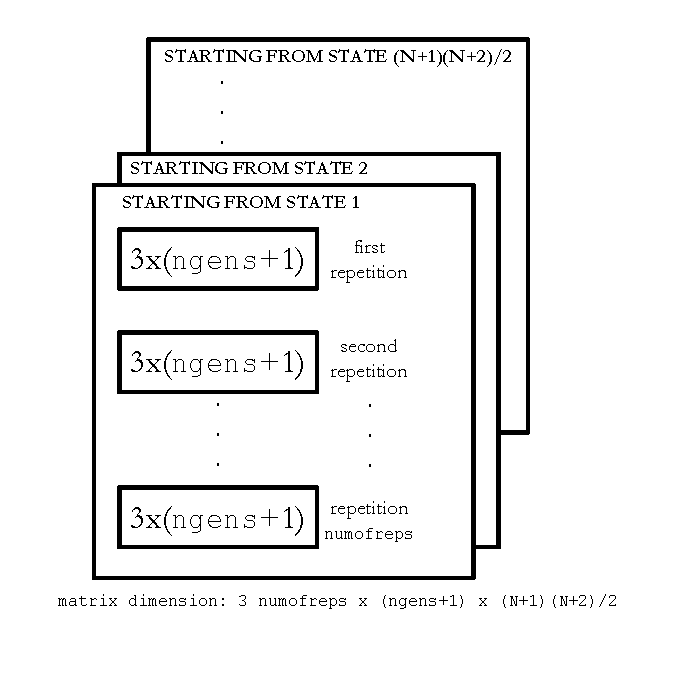
\includegraphics[width=0.6\textwidth]{Matrix Structure.pdf}
    \caption{Structure of the population time evolution matrix.}
\end{figure}
\mintinline{matlab}{populationAnimation(allstatespergenNumOfPlayersHistory(4:6,:,20),chosen,names)} plots the state evolution in time, of the second repetition (4:6), starting from the initial state 20.

\clearpage
\subsection{Function calls}

    

\begin{figure}[h!]
    \centering
    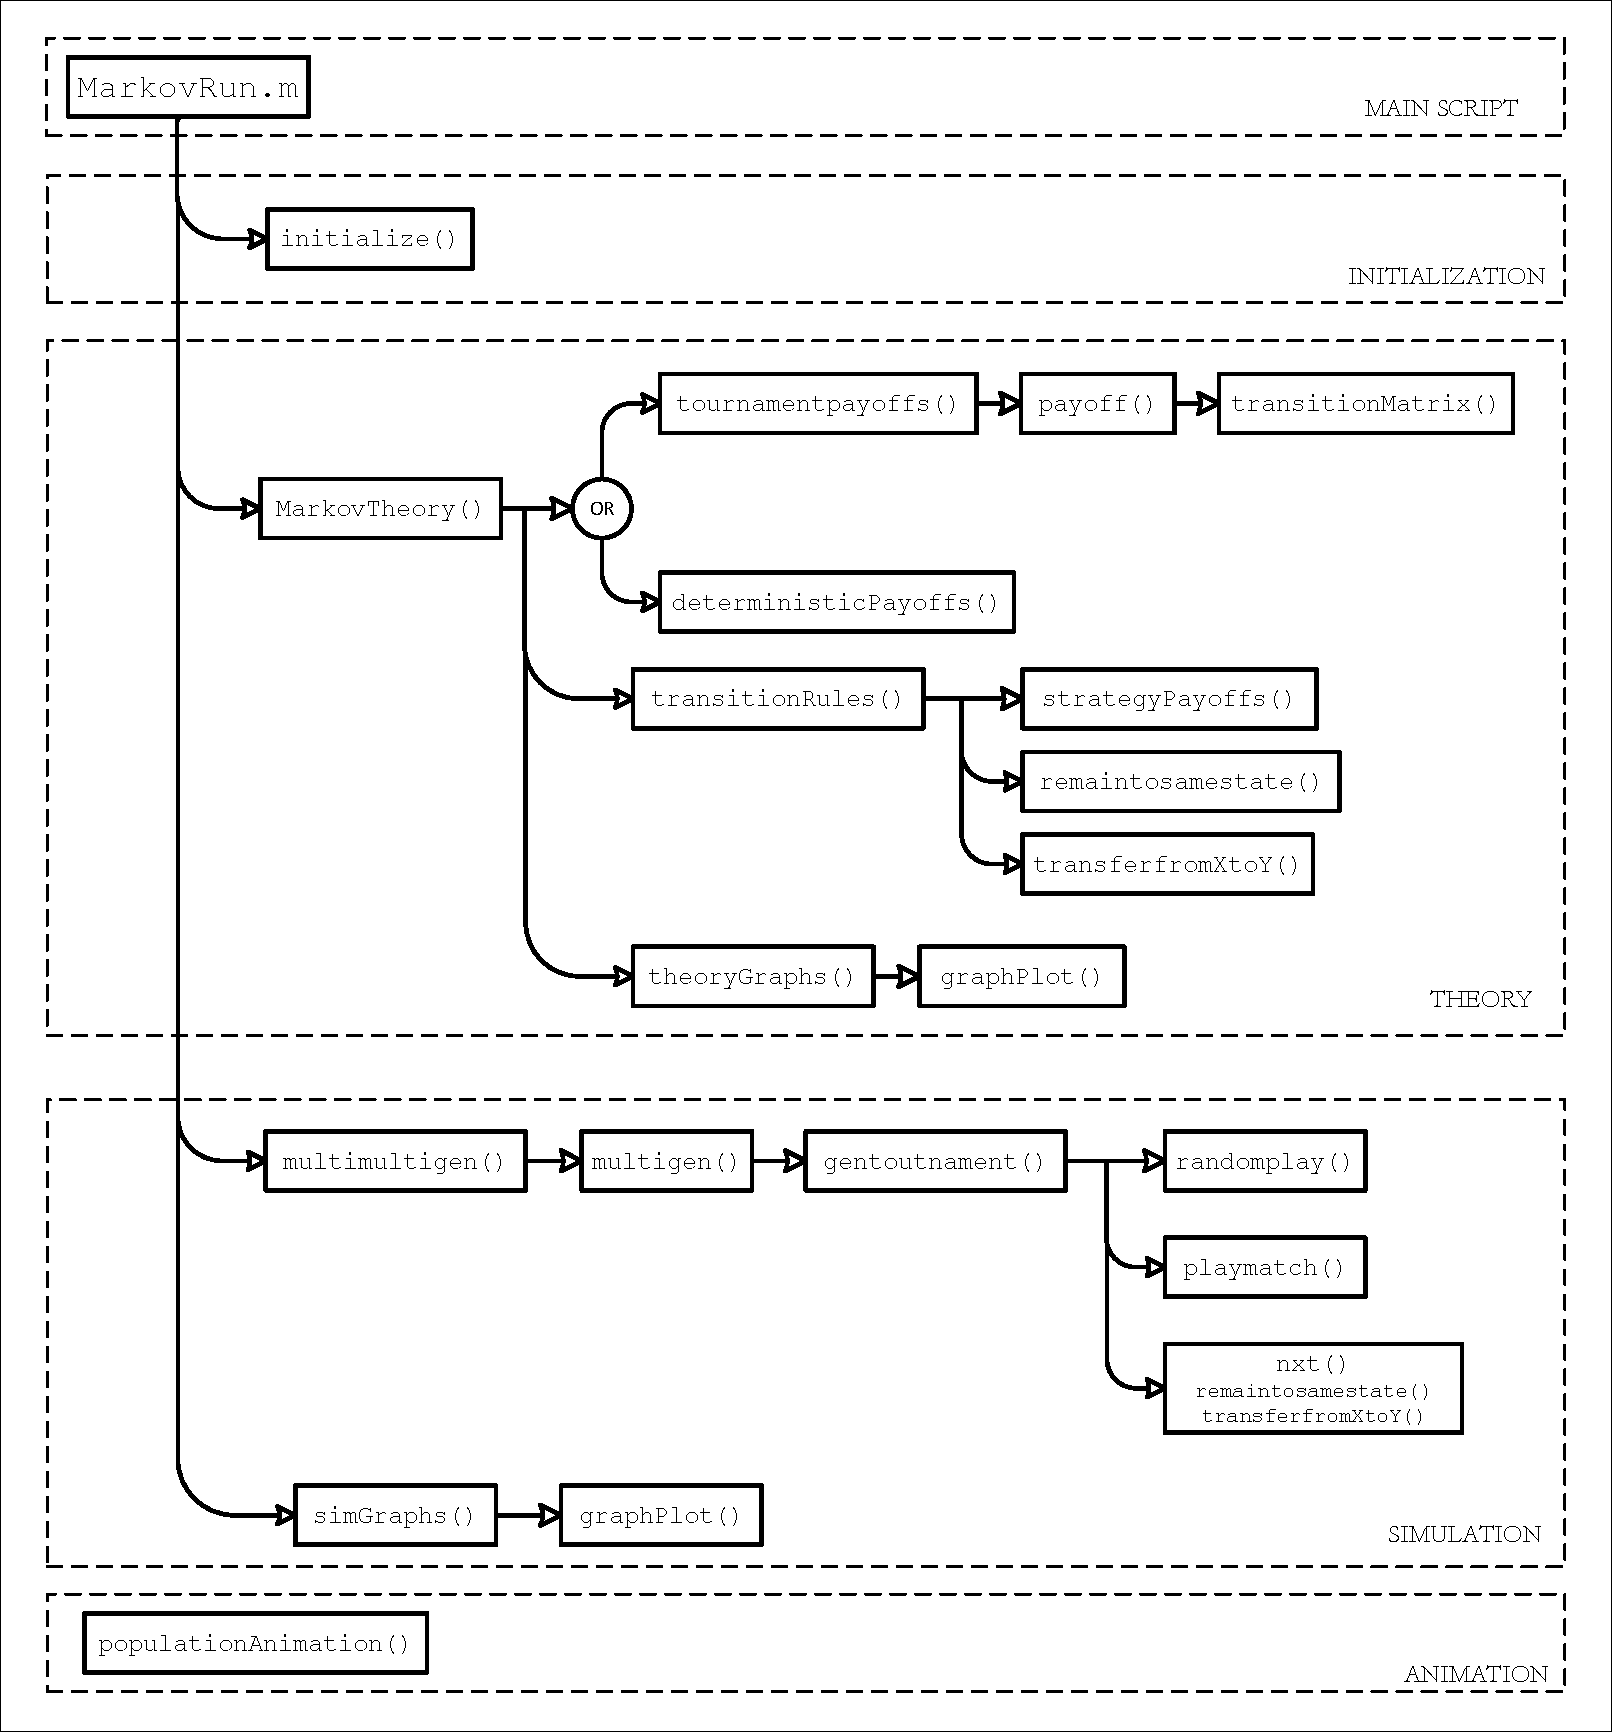
\includegraphics[width=1.15\textwidth]{Function Calls.pdf}
    \caption{Function calls.}
\end{figure}

\chapter{Fitness Dynamics}
\section{Brief Overview}
In the 1999's paper "Studies on Dynamics in the Classical Iterated Prisoner’s Dilemma with Few Strategies" the authors imagine a Prisoner's dilemma like tournament, involving multiple dIfferent strategies. These strategies use a logical basis to derive their move against their opponent, ultimately choosing one out of the two following actions; either cooperate or defect. Each player plays a certain number of rounds with every other player. Once all encounters have been conducted we calculate the strategies' populations to start the next generation. However the encounters between players are not carried out one by one. To expedite the calculations of the Theoretical Fitness Axelrod Genetic Tournament, as we call it, we utilize the fact that when deterministic strategies play with each other, the emerging individual scores are always the same. Thus we can safely emerge to the score of each strategy by following the equation \ref{eq:gnA}.
\begin{align}
g_n(\mathbf{A}) &= W_n(\mathbf{A})V(\mathbf{A}|\mathbf{A}) + W_n(\mathbf{B})V(\mathbf{A}|\mathbf{B}) + W_n(\mathbf{C})V(\mathbf{A}|\mathbf{C}) - V(\mathbf{A}|\mathbf{A}) \label{eq:gnA} \\ 
g_n(\mathbf{B}) &= W_n(\mathbf{A})V(\mathbf{B}|\mathbf{A}) + W_n(\mathbf{B})V(\mathbf{B}|\mathbf{B}) + W_n(\mathbf{C})V(\mathbf{B}|\mathbf{C}) - V(\mathbf{B}|\mathbf{B}) \label{eq:gnB} \\
g_n(\mathbf{C}) &= W_n(\mathbf{A})V(\mathbf{C}|\mathbf{A}) + W_n(\mathbf{B})V(\mathbf{C}|\mathbf{B}) + W_n(\mathbf{C})V(\mathbf{C}|\mathbf{C}) - V(\mathbf{C}|\mathbf{C}) \label{eq:gnC} \\
\end{align}

\begin{align}
\mathrm{t}(n) &= W_n(\mathbf{A})g_n(\mathbf{A}) + W_n(\mathbf{B})g_n(\mathbf{B}) + W_n(\mathbf{C})g_n(\mathbf{C})
\end{align}


\begin{align}
W_{n+1}(\mathbf{A}) &= \frac{\Pi W_n(\mathbf{A}) g_n(\mathbf{A})}{\mathrm{t}(n)} \\ \label{eq:fit}
W_{n+1}(\mathbf{B}) &= \frac{\Pi W_n(\mathbf{B}) g_n(\mathbf{B})}{\mathrm{t}(n)} \\
W_{n+1}(\mathbf{C}) &= \frac{\Pi W_n(\mathbf{C}) g_n(\mathbf{C})}{\mathrm{t}(n)}
\end{align}


The acronyms used are explained in detail here:
\begin{itemize}
\item $g_n(A)$: Total score of strategy A per generation, on generation n
\item $V(A|B)$: Score awarded to A when A encounters B
\item $W_n(A)$: Population of strategy A, on generation n
\item $t(n)$: The sum of the strategies' scores, on generation n
\end{itemize}

To enrich the Theoretical tournament we created two more ways to simulate a Tournament.
\begin{enumerate}
\item \textbf{Simulated Fitness Axelrod Genetic Tournament:} This is a computationally intensive but 1-to-1 accurate way of running the tournament. We make sure to meet each idividual player object with the other. To calculate the next generation's populations we use a fitness function \ref{eq:fit}.

\item \textbf{Simulated Imitation Axelrod Genetic Tournament} And this is an equally computationally intensive but 1-to-1 accurate way of running the tournament, though the next generation's populations are now calulated through imitation. K in number, randomly selected players, who do not belong to the optimal strategy, change strategy and adopt the the best scoring strategy. In case of multiple best scoring strategies, the picking procedure is made to be random.
\end{enumerate}
\section{Player Class}
The player class encapsulates every attribute and method common to all strategies. The dIfferentiation occurs in the subclasses where we sometimes need to add attributes and/or methods. The move() method is implemented on each individual subclass/strategy. The common player attributes are:
\begin{itemize}
    \item \textbf{index}: The index of the player in the game.
    \item \textbf{score}: The score of the player.
    \item \textbf{history}: A list of the player's moves for each round played (rows) when matched with dIfferent other players (columns) in the game.
    \item \textbf{move}: The move of the player in the current round. Can either be \texttt{0} (cooperate) or \texttt{1} (defect).
\end{itemize}
The methods implemented are simple setters and getter that give other classes of our program access to the attributes of the player class.
\section{Strategies Index}
\subsection{Cooperate Class}
Always cooperates.
\subsection{Defect Class}
Always defects.
\subsection{Random Class}
Makes a random move.
\subsection{TitForTat Class}
First cooperate, afterwards copy your opponent's last move.
\subsection{Grim Class}
Starts by cooperating, switches to permanent defection If the opponent ever defects. It tracks whether each opponent has defected using a flag array.
\subsection{hard\_tft Class}
Cooperates on the first two moves, defects after at least one defection in the last two rounds,
cooperates otherwise.
\subsection{slow\_tft Class}
Cooperates on the first  move, defects after two consecutive defections,
and returns to cooperation after two consecutive cooperations by the opponent.
\subsection{tf2t Class}
Tit for 2 tat: Cooperates on the first move, defects after two consecutive opponent defections,
cooperates otherwise.
\subsection{mistrust Class}
Defects on first move, then play what the opponent played on the previous move.
\subsection{pavlov Class}
Cooperates on the first move, then cooperates only If the two players made the same move.
\subsection{per\_CD Class}
Periodically plays cooperate,defect.
\subsection{per\_kind Class}
Periodically plays cooperate, cooperate, defect.
\subsection{per\_nasty Class}
Periodically plays defect, defect, cooperate.
\subsection{gradual Class}
Cooperates on the first move, then defects n times after nth defections
and calms down its opponent with two cooperations.

\begin{algorithm}
\caption{Gradual Strategy}
\begin{algorithmic}[1]

\State For each opponent, track:
\State \quad \textbf{total defections}
\State \quad \textbf{how many punishments remain}
\State \quad \textbf{how many calming cooperations remain}

\Function{SetMove}{opponent's last move, opponent index, current round}

\If{first round}
    \State Cooperate
    \Return
\EndIf

\If{opponent defected}
    \State Increase total defections
\EndIf

\If{currently punishing}
    \State Defect
    \State Decrease punish count
    \Return
\EndIf

\If{currently calming}
    \State Cooperate
    \State Decrease calm count
    \Return
\EndIf

\If{opponent just defected}
    \State Start punishing: defect as many times as total defections so far minus 1
    \State Then plan 2 calming cooperations
    \State Defect
    \Return
\EndIf

\State Cooperate (default behavior)

\EndFunction

\end{algorithmic}
\end{algorithm}


\subsection{soft\_majo Class}
Plays the opponent's most played move, cooperates in case of equality.
\subsection{per\_ccccd Class}
Periodically plays cooperate, cooperate, cooperate, cooperate, defect.
\subsection{prober Class}
Initially plays defect, cooperate, cooperate. On the third cooperate ascertains if the has opponent retaliated on rounds 2 and 3. If yes then the opponent isn't exploitable, thus continue as a tit-for-tat player. Otherwise the opponent is exploitable, thus continue as a defect player to maximize profits.
\begin{algorithm}
\caption{Prober Strategy: Brief overview}
\begin{algorithmic}[1]
\State For each opponent, keep:
\State \quad \textbf{State}: what step we are in
\State \quad \textbf{flag}: whether the opponent is gullible

\Function{SetMove}{opponent's last move, opponent index}

\If{State is 0}
    \State Defect
    \State Go to State 1
\ElsIf{State is 1}
    \State Cooperate
    \State Go to State 2
\ElsIf{State is 2}
    \State Cooperate
    \If{opponent defected}
        \State Mark opponent as gullible
    \EndIf
    \State Go to State 3
\ElsIf{State is 3}
    \If{opponent defected}
        \State Mark opponent as gullible
    \EndIf

    \If{opponent is gullible}
        \State Switch to tit-for-tat (copy opponent's move)
        \State Go to State 4
    \Else
        \State Switch to always defect
        \State Go to State 5
    \EndIf
\ElsIf{State is 4}
    \State Play tit-for-tat (copy opponent's last move)
\ElsIf{State is 5}
    \State Always defect
\EndIf

\EndFunction
\end{algorithmic}    
\end{algorithm}
\newpage
\section{Axelrod Class}
The Axelrod class plays out one generation of the game which comprises of a number of rounds. The class is initialized with the following parameters:
\begin{itemize}
    \item \textbf{players}: A list of players that belong to  play the game.
    \item \textbf{rounds}: The number of rounds the game is played.
    \item \textbf{currentRound}: The current round of the game.
    \item \textbf{payoffMatrix}: The matrix used to calculate the scores of the players based on their moves.
\end{itemize}
The methods of the class include the standard setters and getters but also materializes the main game loop. At first we set the current round and play the round using the \texttt{playRound()} method.
\begin{algorithm}
\caption{\texttt{playRound()} logic}
\begin{algorithmic}
\Function{playRound}{}
  \For{$i \gets 0$ to $N-1$}
    \For{$j \gets i+1$ to $N$}
      \State Run the round between player $i$ and player $j$
    \EndFor
  \EndFor
\EndFunction
\end{algorithmic}
\end{algorithm}


The \texttt{playRound()} logic can be seen below.\\We run two nested loops to effectively simulating all encounters between players. It should be noted that the second loop begins at \texttt{i+1} to avoid enacting the same encounter twice.\\
Finally, the \texttt{encounter()} method is responsible for setting the moves of the two players involved, updating their history column which corresponds to the current round (row) and current opponent (column) and updating their current score.
\begin{algorithm}
\caption{\texttt{encounter()} logic}
\begin{algorithmic}[1]
\Function{encounter}{player1, player2, round}
  \If{round = 1}
   \State each player sets move assuming no history
  \Else 
    \State Each player sets move based on opponent's last move
  \EndIf
  \State Assign payoffs to both players based on moves
  \State Update each player's history with their move     
\EndFunction
\end{algorithmic}
\end{algorithm}
\\Now, in order to start the tournament, we have to convert the input arguments into actual players. The \texttt{InitPlayers()} method creates a map matching specIfic numbers with strategy constructors. The distinct populations determine how many times each strategy object should be created and the number of rounds contributes to the number of rows the history matrices should have.
\newpage
\begin{algorithm}
\caption{The \texttt{initPlayers() logic}}
\begin{algorithmic}[1]
\State Map strategy numbers to constructor functions
\State $players \gets$ empty list
\For {each $(strategy, count)$ in $(strategiesArray, populationsArray)$}
   \If{strategy is valid}
      \For{$i = 1$ to $count$}
        \State Add new player using constructor(strategy) to $players$
      \EndFor
   \Else
       \State \Call{Error}{Invalid Strategy}
   \EndIf
\EndFor
\For{$i = 1$ to length($players$)}
\State Set $players[i].index \gets i$
\State Initialize history for $players[i]$
\EndFor
\State \Return $players$
\end{algorithmic}
\end{algorithm}
\section{Genaxel Class}
With the \texttt{genaxel} class, we simulate and analyze strategy evolution within the Axelrod tournament. The implementation facilitates dIfferent modes of
fitness calculation and evolutionary dynamics.It also supports multiple tournament styles and population update mechanisms.\\
To begin with, the \texttt{TheoreticalFitness} function simulates evolutionary fitness for a population of strategies by conducting pairwise Axelrod tournaments. It computes a score matrix \texttt{V} where each strategy plays against every other, calculates a fitness score \texttt{Gn} for each strategy based on its interactions and current population, and then updates the next generation population \texttt{Wn} propportionally. The function supports multiple rounding schemes, which we explore further down in this report.\\
On the contrary, the \texttt{SimFitness} function collects indivisual scores for each strategy, and aggregates these to compute a total score. Based on each strategy's share of the total score, the function updates the population vector \texttt{Wn} for the next generation, scaling and rounding the values proportionally. This models evolutionary selection based on realtive performance in a full-population tournament setting.\\
Finally, in the \texttt{ImitationSim} function, each strategy's total score is calculated based on its interactions with others and normalized per individual to get average player scores. The strategy with the highest average score is identIfied, and up to  \texttt{K} indivisuals from other non-zero populations are converted to imitate this best-performing strategy. This model "learns" by imitation, where successful strategies attract followers over time.
\clearpage
\begin{algorithm}
\caption{TheoreticalFitness logic}
\begin{algorithmic}[1]
\Require obj, b strategies, pop0, T, rounding
\Ensure obj, Wn, V
\State Initialize $V \gets $ payoff Matrix through oneVone , $Wn \gets pop0$, $Gn \gets 0$, $Tn \gets 0$
\State $totalPlayers \gets \sum Wn$

\For{$i = 1$ to $|\texttt{strategies}|$}
  \For{$j = 1$ to $|\texttt{strategies}|$}
    \State $V[i][j] \gets$ score of player $i$
    \State $Gn[i] \gets Gn[i] + V[i][j] \cdot Wn[j]$
  \EndFor
  \State $Gn[i] \gets Gn[i] - V[i][j]$
  \State $Tn \gets Tn + Gn[i] \cdot Wn[i]$
\EndFor

\State Compute new $Wn$ using $Gn$, $Tn$, and chosen rounding method

\Return obj, $Wn$, $V$
\end{algorithmic}
\end{algorithm}

\begin{algorithm}
\caption{sim\_fitness logic}
\begin{algorithmic}[1]

\Function{sim\_fitness}{strategies, pop0, T, b}

\State Initialize tournament with strategies and payoffs  
\State Run the tournament

\State Set popscore to zero array  
\State Set totalscore to 0  
\State Set totalplayers to sum of pop0  
\State Set Wn to pop0  
\State Set counter to 1

\For{each strategy i}
    \For{each player in strategy i}
        \State Add player’s score to popscore[i]  
        \State Increase counter by 1  
    \EndFor
    \State Add popscore[i] to totalscore  
\EndFor

\For{each strategy i}
    \State Set Wn[i] to floor(totalplayers * popscore[i] / totalscore)  
\EndFor

\Return Wn
\EndFunction
\end{algorithmic}
\end{algorithm}

\clearpage

\begin{algorithm}
\caption{imitation\_sim logic}
\begin{algorithmic}[1]

\Function{imitation\_sim}{strategies, pop0, K, T, b}

\State Set Wn to pop0  
\State Create empty matrix V[strategy][strategy]  
\State Create score array Gn initialized to zeros  
\State Set oneVone to [1, 1]

\For{each strategy i}
    \For{each strategy j}
        \State Create temporary player list with strategy i and j  
        \State Initialize a new tournament with those players  
        \State Run the tournament  
        \State Set V[i][j] to score of strategy i against strategy j  
        \State Add V[i][j] $\times$ Wn[j] to Gn[i]  
    \EndFor
    \State Subtract V[i][i] from Gn[i]  
\EndFor

\State Set popscore to Gn  
\State Compute average score per player: playerscore[i] = popscore[i] / Wn[i]  

\State Find maximum value in playerscore  
\State Find all indices with that value  
\State Randomly choose one indexBest among them  
\State Set Bestscore to playerscore[indexBest]  
\State Set newIndex to indexBest

\For{i from 1 to K}
    \State Find all zero-population strategy indices  
    \If{there are at least two non-zero populations}
        \While{newIndex equals indexBest or newIndex in zero-population list}
            \State Select newIndex randomly from strategies  
        \EndWhile
        \State Decrease Wn[newIndex] by 1  
        \State Increase Wn[indexBest] by 1  
        \State Reset newIndex to indexBest  
    \EndIf
\EndFor

\Return Wn

\EndFunction
\end{algorithmic}
\end{algorithm}
We noticed that the way we implemented \texttt{genaxel} was time consuming, because of recurring initialization of Axelrod tournament wich essentially calculated time and again th epayoff Matrix, \texttt{V}.\\
In the following, improved version, we made the function "oneVone" which is only called once, at the beginning of \texttt{genaxel} in \texttt{TourTheFit()}.
\newpage
\begin{algorithm}
\caption{one\_v\_one}
\begin{algorithmic}[1]

\Function{one\_v\_one}{strategies, T, b}

\State Create matrix V of zeros with size [strategies][strategies]  
\State Set population array to [1, 1]

\For{each strategy i}
    \For{each strategy j}
        \State Create temporary pair [strategy i, strategy j]  
        \State Initialize a new tournament with that pair  
        \State Run the tournament  
        \State Set V[i][j] to the score of player 1  
    \EndFor
\EndFor

\State Store V in object  
\State \textbf{return} V
\EndFunction
\end{algorithmic}
\end{algorithm}




\clearpage
\section{Script}
The Script is our means to configure the program and the dIfferent kinds of tournaments we engineered. Through the script one can edit the following paramenters:
\begin{itemize}
    \item \texttt{sim\_mode}: The simulation mode. Can take one of 4 values:
        \begin{itemize}
            \item \texttt{Axel}: Axelrod, is a simple Axelrod tournament.
            \item \texttt{TourTheFit}: Tournament Theoretical Fitness, is a genetic algorithm implementing the Axelrod tournament for many generations. The mechanism for determining the next generation includes finding the ratio of the total score each strategy accumulated and distributing the total number of players to the individual strategies based on that ratio. The encounters here are only theoretical. We save on computation time by encountering the strategies and multiplying by their populations. 
            \item \texttt{TourSimFit}: Tournament Simulated Fitness, is a genetic algorithm implementing the Axelrod tournament for many generations. This algorithm's mechanism is the same as TourTheFit but this time the players have to be distinct and truly encounter one another. More computationally expensive but also able to accurately simulate random strategies.
            \item \texttt{TourSimImit}: Tournament Simulated Imitation, genetic algorithm implementing the Axelrod tournament for many generations. The mechanism for determining the next generation has the suboptimal players converting to the best performing strategy.
        \end{itemize}
    \item \texttt{meeting\_mode}: Meeting mode, lets the user choose from a number of dIfferent meetings created as experiments by the authors of "" to highlight various interesting emerging States.
\end{itemize}

The user is also able to run custom tournaments by selecting the custom meeting mode and thereafter changing any of the following parameters:
\begin{itemize}
    \item \textbf{strategies}: The strategies participating in the tournament. 
    \item \textbf{populations}: The populations of each strategy.
    \item \textbf{payoffMatrix}: The matrix that determines the scores of the players.
    \item \textbf{rounds}: The number of rounds to be played each generation of the tournament.
    \item \textbf{generations}: The number of generations to be played in the tournament.
    \item \textbf{rounding}: The rounding method used to have integer populations each generations while, also, keeping the initial total population.
    \item \textbf{K}: The number of players that will imitate the best performing strategy.
\end{itemize}
Running the script.m file runs the tournament with the parameters set inside it. The results are plotted for visualization.

\section{Meetings}
Retaining the exact same number of players, each generation, requires rounding up the emerging number of players each strategy has at the end of each generation and then redistributing the decimal parts. Ultimately, the decimal parts in our 3-strategy meetings add up to either one or two, and the distribution method we found to be the most fair was:
\begin{itemize}
    \item If the remainder sum is 1, we round up each strategy to the previous integer and distribute the decimal part to the strategy that is the closest to its next integer.
    \item If the remainder sum is 2, we round up each strategy to the previous integer and distribute the decimal part to the two strategies that are the closest to their next integer. 1 to each.
    \item If the remainder sum is 0, there are no decimal parts.
\end{itemize}
We also devised a similar method which, this time, distributes the decimal parts to the top two strategies in terms of total population. We used both methodologies to conduct our experiments. However, when comparing our results with the 1999's paper "Studies on Dynamics in the Classical Iterated Prisoner's Dilemma with Few Strategies" the graphs we produced were mostly coherent but ultimately dIfferent. These dIfferences can be largely attributed to the mutable nature of the simulations hidden in programming layers of abstraction and the non-disclosed method of rounding used by the authors of the paper. They only Stated that: "All divisions being rounded to the nearest lower integer.", which is not accurate based on their results which seem to be retaining their initial total population. This will be an attempt to replicate the paper's results while attributing our dIfferences and trying to make the same point the original authors were trying to make regardless of the dIfferences. Our rounding logic is presented in the next page.
\begin{algorithm}
\caption{Decimal redistribution logic}
\begin{algorithmic}[1]
\If{rounding is paper}
  \For{each strategy}
      \State Calculate share of players
      \State Round down to nearest whole number
  \EndFor
\EndIf

\If{rounding is pop}
  \For{each strategy}
      \State Calculate share of players
      \State Save the decimal part
      \State Round down to whole number
  \EndFor
  \State Count how many players have to be redistributed
  \State Sort strategies by largest population count
  \For{each leftover player} 
    \State Give to strategies ranking highest
  \EndFor
\EndIf

\If{rounding is dec}
  \For{each strategy}
      \State Calculate share of players
      \State Save the decimal part
      \State Round down to whole number
  \EndFor
  \State Count how many players have to be redistributed 
  \State Sort strategies by largest decimal part
  \For{each leftover player} 
    \State Give to strategy with largest decimal
  \EndFor
\EndIf

\If{rounding is off}
  \For{each strategy}
      \State Just calculate  the exact, non-rounded share
  \EndFor
\EndIf    
\end{algorithmic}
\end{algorithm}


It is important to note that when comparing equal quantities there is no clear ranking between remainders. Thus the program decides where to distribute the decimal parts based on the order of the strategies. This could very well be consequential enough to skew the results in a different direction. Let's see how our results compare relative to the ones in the paper. Along with our own rounding methods we managed to reverse engineer the paper's method. It involves pinning the total population at the start of the code so as to only compute the strategies' score ratios. We then floor the emerging individual populations but no matter the decimal parts the total population of each round cannot become 
    $\leq constant\_total\_population-3$. Since the results are exactly the same there isn't any commentation to be done. Thus we will only depict them as proof we recreated the paper's results.
\newpage

%%%%%%%%%%%%%%%%%%%%%%%%% Meetings %%%%%%%%%%%%%%%%%%%%%%%%%%%%%%%%
%%%%%%%%%%%%%%%%%%%%%%%%%%%%%%%%%%%%%%%%%%%%%%%%%%%%%%%%%%%%%%%%%%%
\subsection{Defectors may be strong}
This meeting is supposed to show how defecting more often can be beneficial, for the defector, in chaotic environments. When rounding using the "off" method soft majority does not get eradicated leading to different behavior. Same are the results we get with the "dec" method too, only this time we increase the number of generations to observe the entire phenomenon. It is evident that the oscillations converge to a stable periodic State.
\begin{figure}[H]
    \centering
    \begin{minipage}[c]{0.58\textwidth}
        \centering
        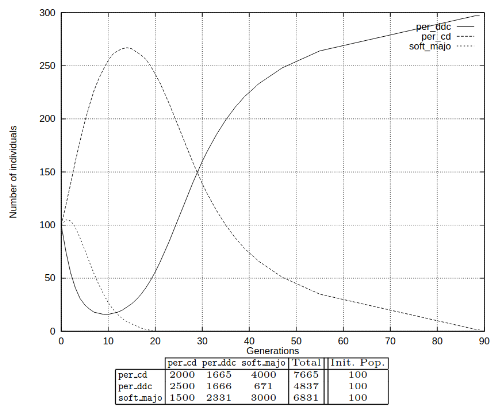
\includegraphics[width=\textwidth]{defectors_may_be_strong.png}
        \caption{Defectors may be strong Original Plot}
    \end{minipage}
    \hfill
    \begin{minipage}[c]{0.4\textwidth}
        \centering
        \begin{tabular}{|l|c|} 
        \hline
        \textbf{Strategy}  & \textbf{Population} \\
        \hline
        soft\_majo   & 100 \\
        per\_cd      & 100 \\
        per\_ddc     & 100 \\
        \hline
        \multicolumn{2}{|l|}{\textbf{Notes:}} \\
        \multicolumn{2}{|l|}{Rounds = 1000} \\
        \multicolumn{2}{|l|}{Generations = 90} \\
        \multicolumn{2}{|l|}{Matrix = \(\begin{bmatrix} 3 & 0 \\ 5 & 1 \end{bmatrix}\)} \\
        \hline
        \end{tabular}
        \captionof{table}{Initial populations}
    \end{minipage}
\end{figure}
\begin{figure}[H]
    \centering
    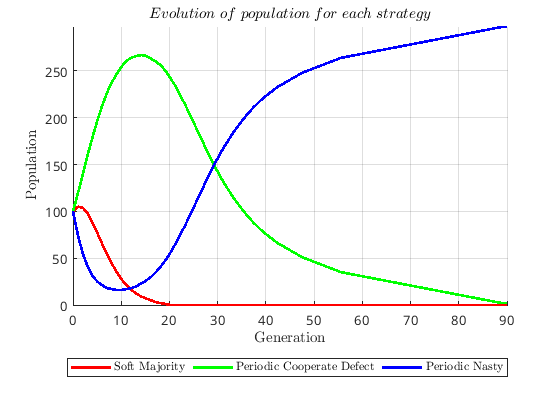
\includegraphics[width=0.8\textwidth]{defectors_may_be_strong_paper.png}
    \caption{Defectors may be strong Paper Plot}
\end{figure}
\begin{figure}[H]
    \centering
    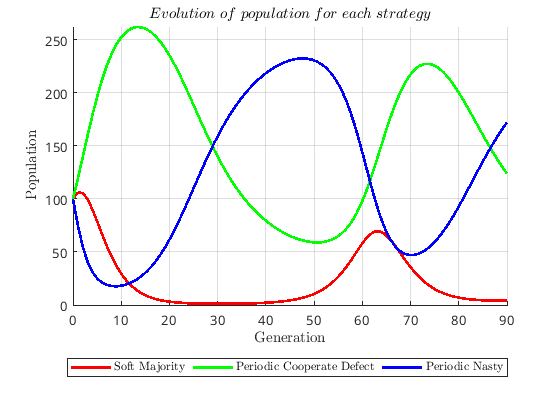
\includegraphics[width=0.8\textwidth]{defectors_may_be_strong_off.png}
    \caption{Defectors may be strong Off Plot}
\end{figure}
\begin{figure}[H]
    \centering
    \includegraphics[width=0.8\textwidth]{defectors_may_be_strong_dec.png}
    \caption{Defectors may be strong Dec Plot}
\end{figure}
When rounding using the "pop" method we replicate the results of the paper.
\begin{figure}[H]
    \centering
    \includegraphics[width=0.8\textwidth]{defectors_may_be_strong_pop.png}
    \caption{Defectors may be strong Pop Plot}
\end{figure}


\newpage
\subsection{Monotonous convergence}
This meeting simulates clear monotonous convergence. The paper claims this is the most common outcome of the experiments they ran. Here all methods "pop", "dec" and "off" methods produced identical results recreating the paper's plots.
\begin{figure}[H]
    \centering
    \begin{minipage}[c]{0.58\textwidth}
        \centering
        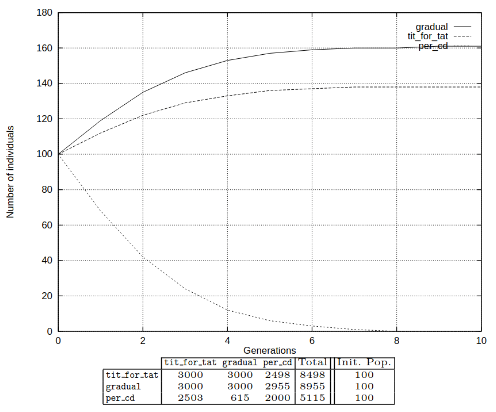
\includegraphics[width=0.8\textwidth]{monotonous_convergence.png}
        \caption{Monotonous convergence Original Plot}
    \end{minipage}
    \hfill
    \begin{minipage}[c]{0.4\textwidth}
        \centering
        \begin{tabular}{|l|c|} 
        \hline
        \textbf{Strategy}  & \textbf{Population} \\
        \hline
        tft          & 100 \\
        per\_cd      & 100 \\
        gradual      & 100 \\
        \hline
        \multicolumn{2}{|l|}{Rounds = 1000} \\
        \multicolumn{2}{|l|}{Generations = 10} \\
        \multicolumn{2}{|l|}{Matrix = \(\begin{bmatrix} 3 & 0 \\ 5 & 1 \end{bmatrix}\)} \\
        \hline
        \end{tabular}
        \captionof{table}{Initial populations}
    \end{minipage}
\end{figure}

\begin{figure}[H]
    \centering
    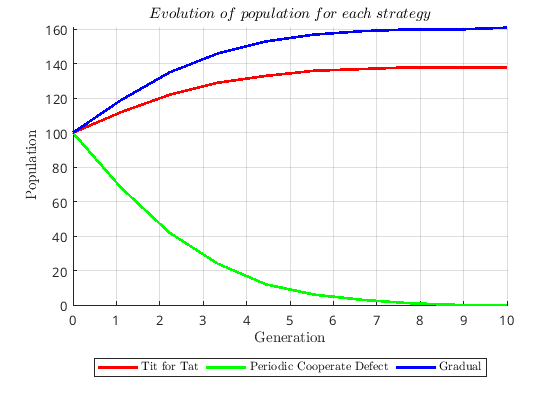
\includegraphics[width=0.8\textwidth]{monotonous_convergence_paper.png}
    \caption{Monotonous convergence Paper Plot}
\end{figure}
\begin{figure}[H]
    \centering
    \includegraphics[width=0.8\textwidth]{monotonous_convergence_dec.png}
    \caption{Monotonous convergence Dec Plot}
\end{figure}
\begin{figure}[H]
    \centering
    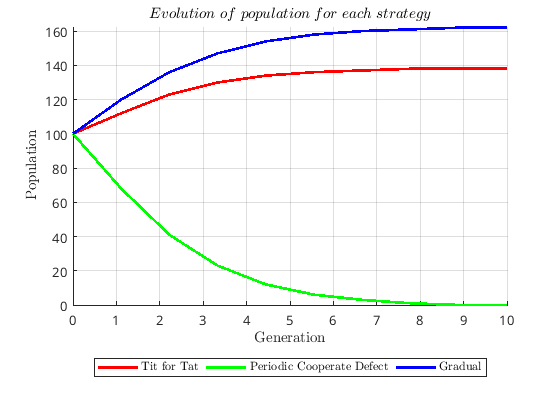
\includegraphics[width=0.8\textwidth]{monotonous_convergence_pop.png}
    \caption{Monotonous convergence Pop Plot}
\end{figure}
\begin{figure}[H]
    \centering
    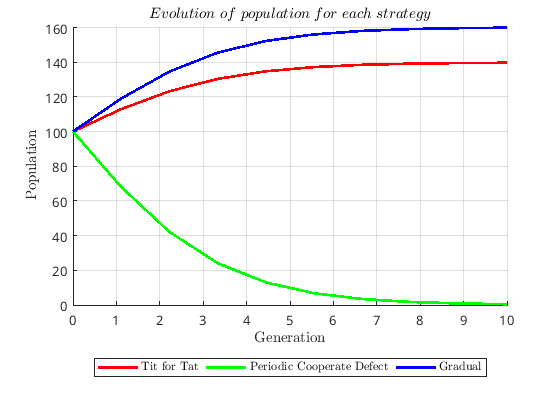
\includegraphics[width=0.8\textwidth]{monotonous_convergence_off.png}
    \caption{Monotonous convergence Off Plot}
\end{figure}

\newpage
\subsection{Attenuated oscillatory movements}
Here we see decreasing oscillations that reach an equilibrium. All rounding methods are again very close to the paper.
\begin{figure}[H]
    \centering
    \begin{minipage}[c]{0.58\textwidth}
        \centering
        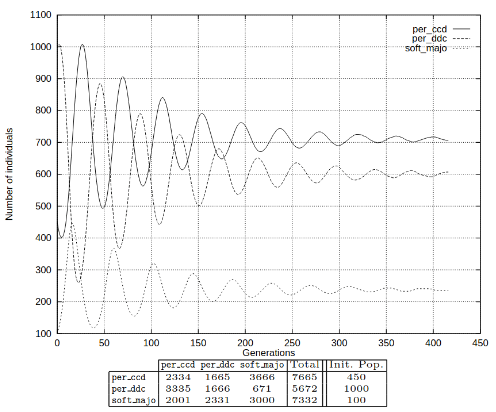
\includegraphics[width=0.8\textwidth]{attenuated_oscillatory_movements.png}
        \caption{Attenuated oscillatory movements Original Plot}
    \end{minipage}
    \hfill
    \begin{minipage}[c]{0.4\textwidth}
        \centering
        \begin{tabular}{|l|c|} 
        \hline
        \textbf{Strategy}  & \textbf{Population} \\
        \hline
        soft\_majo    & 100 \\
        per\_ccd      & 450 \\
        per\_ddc      & 1000 \\
        \hline
        \multicolumn{2}{|l|}{Rounds = 1000} \\
        \multicolumn{2}{|l|}{Generations = 450} \\
        \multicolumn{2}{|l|}{Matrix = \(\begin{bmatrix} 3 & 0 \\ 5 & 1 \end{bmatrix}\)} \\
        \hline
        \end{tabular}
        \captionof{table}{Initial populations}
    \end{minipage}
\end{figure}

\begin{figure}[H]
    \centering
    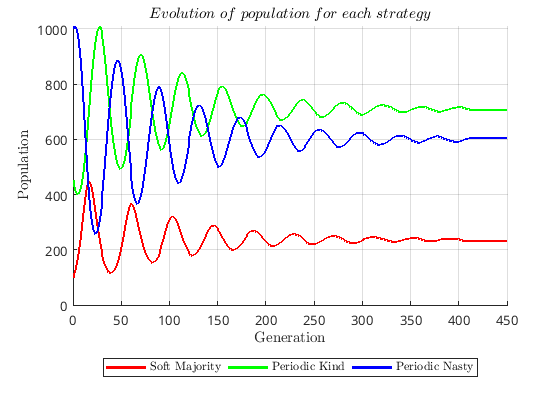
\includegraphics[width=0.8\textwidth]{attenuated_oscillatory_movements_paper.png}
    \caption{Attenuated oscillatory movements Paper Plot}
\end{figure}
\begin{figure}[H]
    \centering
    \includegraphics[width=0.8\textwidth]{attenuated_oscillatory_movements_dec.png}
    \caption{Attenuated oscillatory movements Dec Plot}
\end{figure}
\begin{figure}[H]
    \centering
    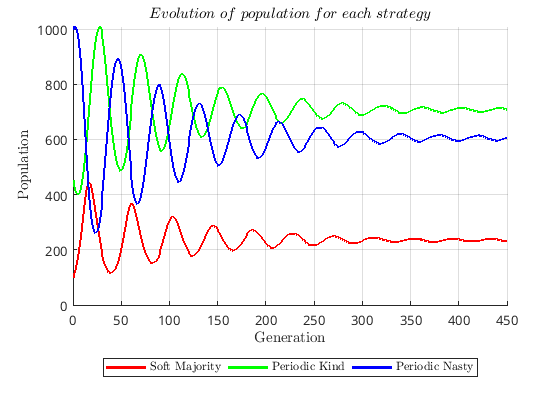
\includegraphics[width=0.8\textwidth]{attenuated_oscillatory_movements_pop.png}
    \caption{Attenuated oscillatory movements Pop Plot}
\end{figure}
\begin{figure}[H]
    \centering
    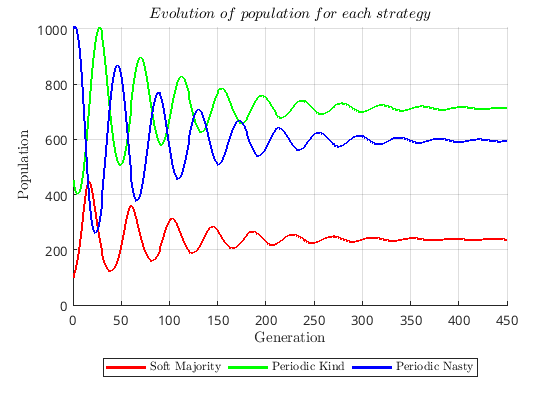
\includegraphics[width=0.8\textwidth]{attenuated_oscillatory_movements_off.png}
    \caption{Attenuated oscillatory movements Off Plot}
\end{figure}

\newpage
\subsection{Periodic movements}
The periodic movements meeting highlights the periodicity and constant amplitude of the oscillations. The "dec" rounding method comes closest to replicating the paper's results. The "pop" method produces oscillations that overlap due to the oscillations' bigger amplitude. Finally, the "off" method creates oscillations that soon enough reach to a stable State.
\begin{figure}[H]
    \centering
    \begin{minipage}[c]{0.58\textwidth}
        \centering
        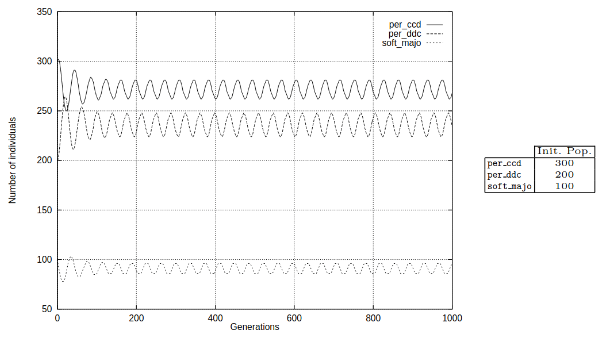
\includegraphics[width=0.8\textwidth]{periodic_movements.png}
        \caption{Periodic movements Original Plot}
    \end{minipage}
    \hfill
    \begin{minipage}[c]{0.4\textwidth}
        \centering
        \begin{tabular}{|l|c|} 
        \hline
        \textbf{Strategy}  & \textbf{Population} \\
        \hline
        soft\_majo    & 100 \\
        per\_ccd      & 300 \\
        per\_ddc      & 200 \\
        \hline
        \multicolumn{2}{|l|}{Rounds = 1000} \\
        \multicolumn{2}{|l|}{Generations = 1000} \\
        \multicolumn{2}{|l|}{Matrix = \(\begin{bmatrix} 3 & 0 \\ 5 & 1 \end{bmatrix}\)} \\
        \hline
        \end{tabular}
        \captionof{table}{Initial populations}
    \end{minipage}
\end{figure}

\begin{figure}[H]
    \centering
    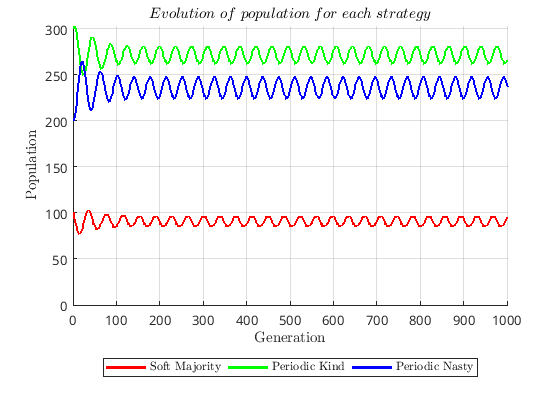
\includegraphics[width=0.8\textwidth]{periodic_movements_paper.png}
    \caption{Periodic movements Paper Plot}
\end{figure}
\begin{figure}[H]
    \centering
    \includegraphics[width=0.8\textwidth]{periodic_movements_dec.png}
    \caption{Periodic movements Dec Plot}
\end{figure}
Using the "pop" method increased the amplitude of the oscillations.
\begin{figure}[H]
    \centering
    \includegraphics[width=0.8\textwidth]{periodic_movements_pop.png}
    \caption{Periodic movements Pop Plot}
\end{figure}
\begin{figure}[H]
    \centering
    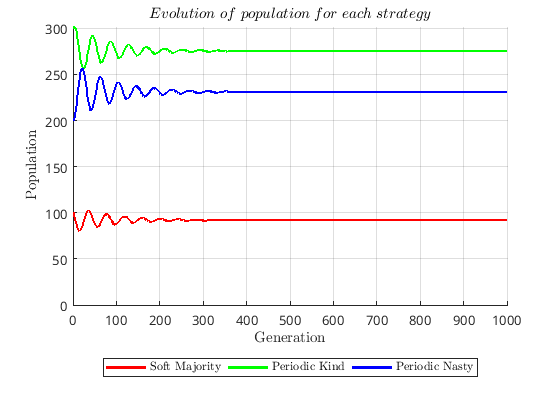
\includegraphics[width=0.8\textwidth]{periodic_movements_off.png}
    \caption{Periodic movements Off Plot}
\end{figure}

\newpage
\subsection{Increasing oscillations}
The increasing oscillations effect in an environment where the total players remain constant can be attributed to Periodic Nasty and Periodic Cooperate Defect who seem to be getting their extra population from driving soft majority into extinction and from being out of phase with each other. "dec" and "off" methods seem be following the attenuated oscillatory movements wand the "pop" method is a bit slower at converging.
\begin{figure}[H]
    \centering
    \begin{minipage}[c]{0.58\textwidth}
        \centering
        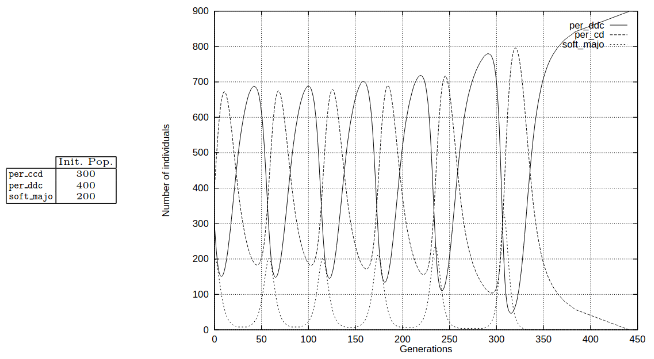
\includegraphics[width=0.8\textwidth]{increasing_oscillations.png}
        \caption{Increasing oscillations Original Plot}
    \end{minipage}
    \hfill
    \begin{minipage}[c]{0.4\textwidth}
        \centering
        \begin{tabular}{|l|c|} 
        \hline
        \textbf{Strategy}  & \textbf{Population} \\
        \hline
        soft\_majo    & 200 \\
        per\_cd       & 400 \\
        per\_ddc      & 300 \\
        \hline
        \multicolumn{2}{|l|}{Rounds = 1000} \\
        \multicolumn{2}{|l|}{Generations = 450} \\
        \multicolumn{2}{|l|}{Matrix = \(\begin{bmatrix} 3 & 0 \\ 5 & 1 \end{bmatrix}\)} \\
        \hline
        \end{tabular}
        \captionof{table}{Initial populations}
    \end{minipage}
\end{figure}

\begin{figure}[H]
    \centering
    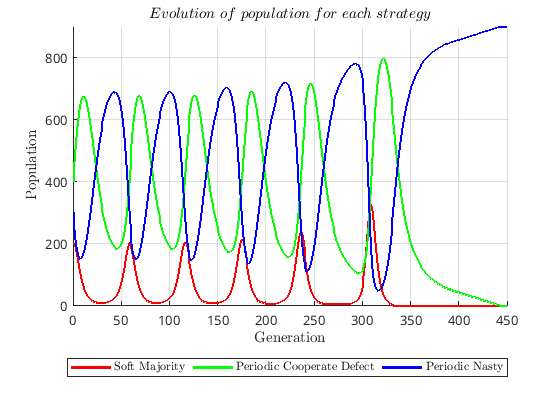
\includegraphics[width=0.8\textwidth]{increasing_oscillations_paper.png}
    \caption{Increasing oscillations Paper Plot}
\end{figure}
\begin{figure}[H]
    \centering
    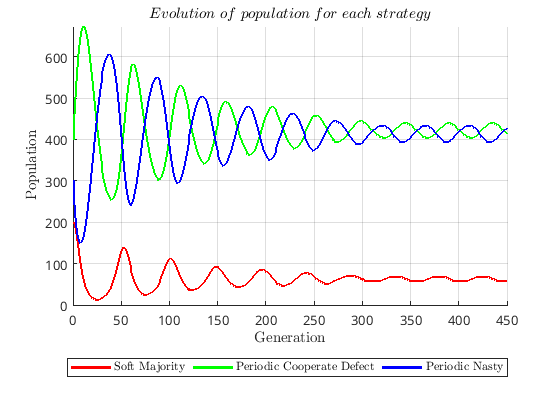
\includegraphics[width=0.8\textwidth]{increasing_oscillations_dec.png}
    \caption{Increasing oscillations Dec Plot}
\end{figure}
\begin{figure}[H]
    \centering
    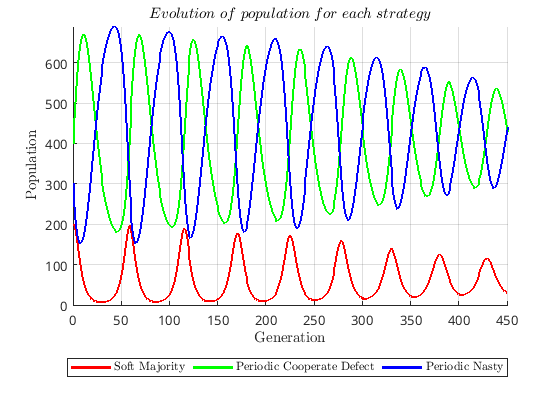
\includegraphics[width=0.8\textwidth]{increasing_oscillations_pop.png}
    \caption{Increasing oscillations Pop Plot}
\end{figure}
\begin{figure}[H]
    \centering
    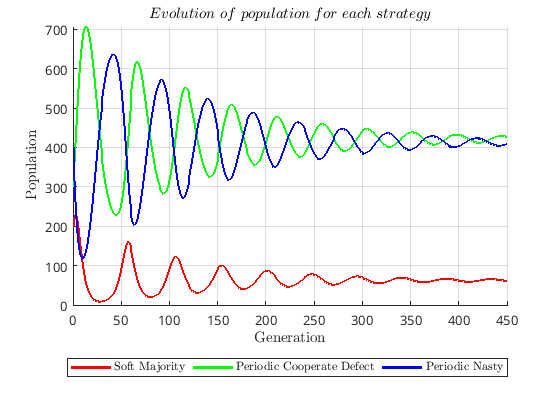
\includegraphics[width=0.8\textwidth]{increasing_oscillations_off.png}
    \caption{Increasing oscillations Off Plot}
\end{figure}

\newpage
\subsection{Disordered oscillations}
When examining the disordered oscillations, "dec" and "off" methods almost recreate the paper's results at a more subtle way. "pop" very quickly concluded its tournament by having soft majority dominate the other two strategies by round 50.
\begin{figure}[H]
    \centering
    \begin{minipage}[c]{0.58\textwidth}
        \centering
        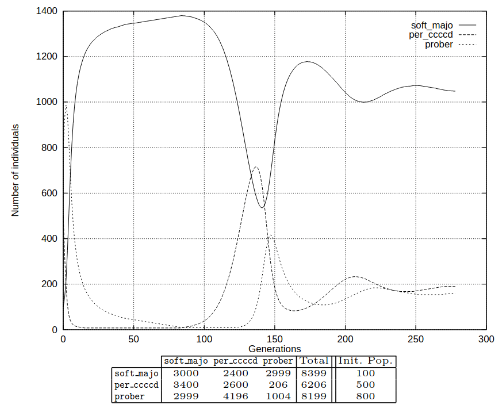
\includegraphics[width=0.8\textwidth]{disordered_oscillations.png}
        \caption{Disordered oscillations Original Plot}
    \end{minipage}
    \hfill
    \begin{minipage}[c]{0.4\textwidth}
        \centering
        \begin{tabular}{|l|c|} 
        \hline
        \textbf{Strategy}  & \textbf{Population} \\
        \hline
        soft\_majo     & 100 \\
        per\_ccccd     & 500 \\
        prober         & 800 \\
        \hline
        \multicolumn{2}{|l|}{Rounds = 1000} \\
        \multicolumn{2}{|l|}{Generations = 300} \\
        \multicolumn{2}{|l|}{Matrix = \(\begin{bmatrix} 3 & 0 \\ 5 & 1 \end{bmatrix}\)} \\
        \hline
        \end{tabular}
        \captionof{table}{Initial populations}
    \end{minipage}
\end{figure}

\begin{figure}[H]
    \centering
    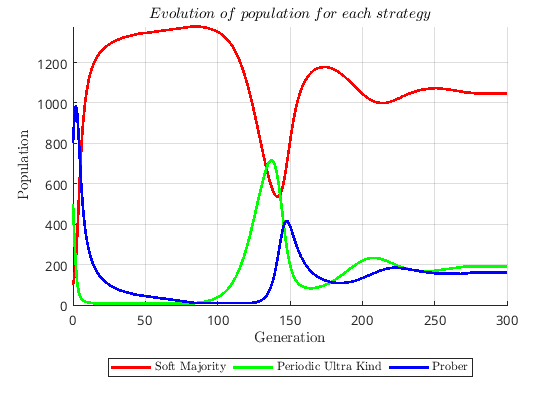
\includegraphics[width=0.8\textwidth]{disordered_oscillations_paper.png}
    \caption{Disordered oscillations Paper Plot}
\end{figure}
\begin{figure}[H]
    \centering
    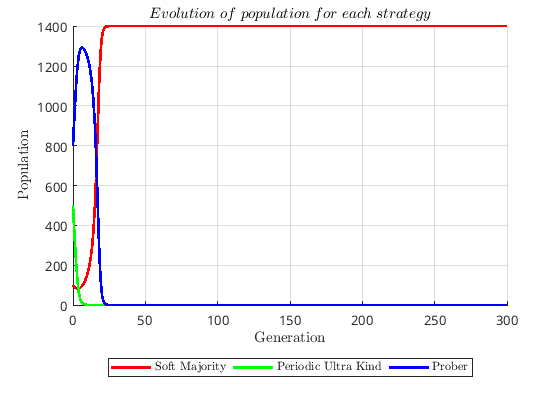
\includegraphics[width=0.8\textwidth]{disordered_oscillations_dec.png}
    \caption{Disordered oscillations Dec Plot}
\end{figure}
\begin{figure}[H]
    \centering
    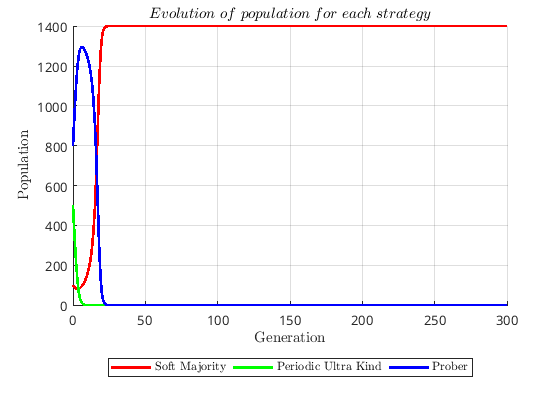
\includegraphics[width=0.8\textwidth]{disordered_oscillations_pop.png}
    \caption{Disordered oscillations Pop Plot}
\end{figure}
\begin{figure}[H]
    \centering
    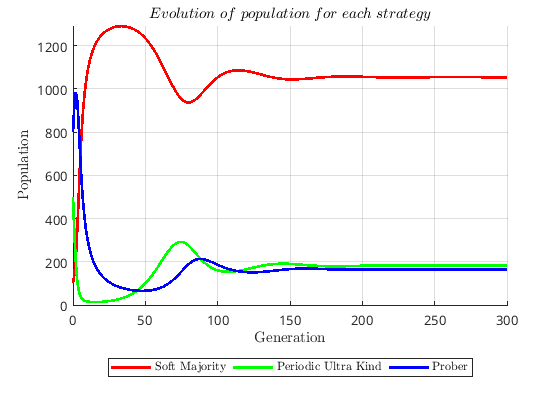
\includegraphics[width=0.8\textwidth]{disordered_oscillations_off.png}
    \caption{Disordered oscillations Off Plot}
\end{figure}

\newpage
\subsection{Population size sensitivity}
Going forward the paper decides to explore the tournament's sensitivity in slight changes of various parameters starting with the initial population size. Other than the fact that the crucial point where the oscillations stop gets shifted at periodic defect-defect-cooperate population: 235 into 236, instead of 244 into 245, the plots "dec" and "pop" recreate the same phenomenon. Furthermore, a pattern that seems to be emerging is the non-oscillating State that the "off" method reaches. This can most likely be attributed to the fact that at some point the distribution of the decimal points becomes periodic in our own methods. "off" which doesn't redistribute the decimal parts has no problem converging to a final state.
\begin{figure}[H]
    \centering
    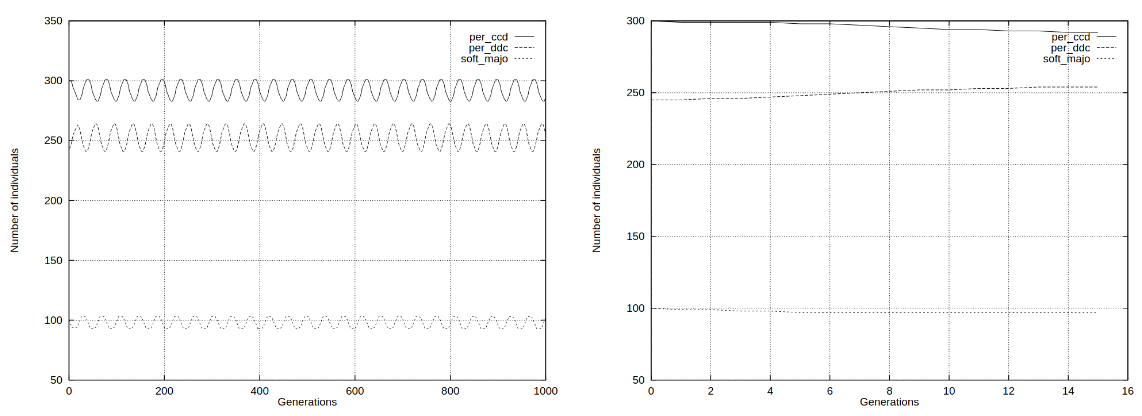
\includegraphics[width=0.8\textwidth]{population_size_sensitivity.png}
    \caption{Population size sensitivity Original Plot}
\end{figure}

\begin{table}[H]
    \centering
    \begin{tabular}{|l|c|}
    \hline
    \textbf{Strategy}  & \textbf{Population} \\
    \hline
    soft\_majo   &  100 \\
    per\_ccd     &  300 \\
    per\_ddc    &  235 (or 244) $\rightarrow$ 236 (or 245) \\
    \hline
    \multicolumn{2}{|l|}{\textbf{Notes:}} \\
        \multicolumn{2}{|l|}{Rounds = 1000} \\
        \multicolumn{2}{|l|}{Generations = 1000 $\rightarrow$ 16} \\
        \multicolumn{2}{|l|}{Matrix = \(\begin{bmatrix} 3 & 0 \\ 5 & 1 \end{bmatrix}\)} \\
    \hline
    \end{tabular}
    \caption{Initial populations}
\end{table}
%%%%%%%%%%%%%%%%%%
\begin{figure}[H]
    \centering
    \begin{subfigure}[t]{0.45\textwidth}
        \centering
        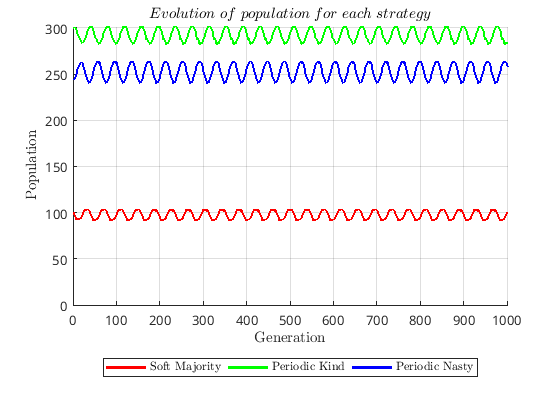
\includegraphics[width=\textwidth]{population_size_sensitivity_before_paper.png}
        \caption{Before}
    \end{subfigure}
    \hfill
    \begin{subfigure}[t]{0.45\textwidth}
        \centering
        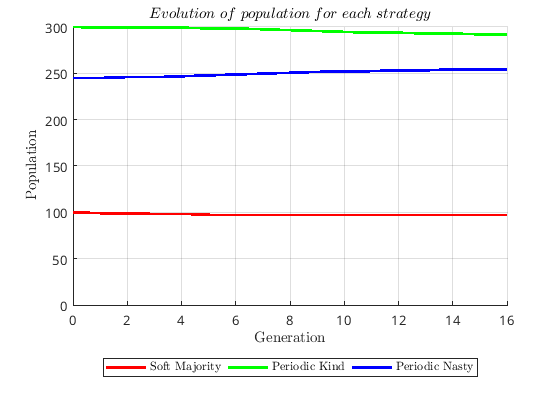
\includegraphics[width=\textwidth]{population_size_sensitivity_after_paper.png}
        \caption{After}
    \end{subfigure}
    \caption{Side-by-side comparison of population size sensitivity before and after Paper}
\end{figure}
%%%%%%%%%%%%%%%%%%%%%%%%%%%%%%%
\begin{figure}[H]
    \centering
    \begin{subfigure}[t]{0.45\textwidth}
        \centering
        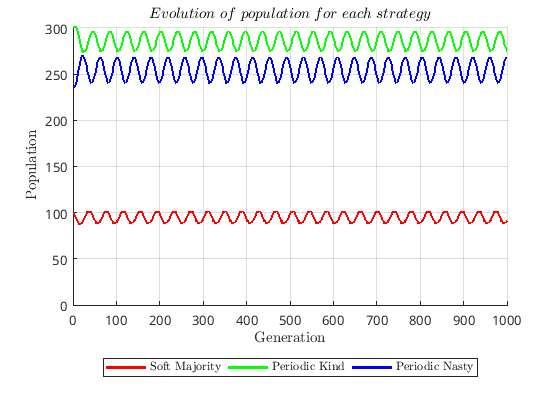
\includegraphics[width=\textwidth]{population_size_sensitivity_before_pop.png}
        \caption{Before}
    \end{subfigure}
    \hfill
    \begin{subfigure}[t]{0.45\textwidth}
        \centering
        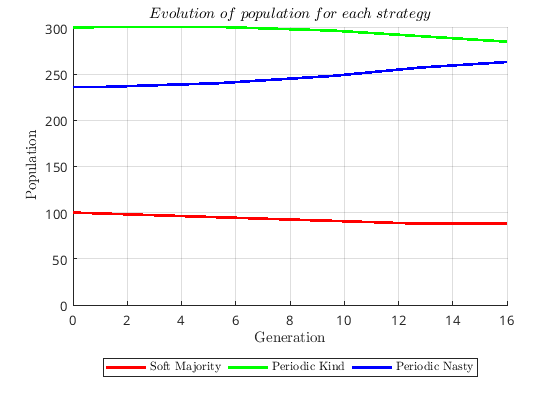
\includegraphics[width=\textwidth]{population_size_sensitivity_after_pop.png}
        \caption{After}
    \end{subfigure}
    \caption{Side-by-side comparison of population size sensitivity before and after Pop}
\end{figure}
\begin{figure}[H]
    \centering
    \begin{subfigure}[t]{0.45\textwidth}
        \centering
        \includegraphics[width=\textwidth]{population_size_sensitivity_before_dec.png}
        \caption{Before}
    \end{subfigure}
    \hfill
    \begin{subfigure}[t]{0.45\textwidth}
        \centering
        \includegraphics[width=\textwidth]{population_size_sensitivity_after_dec.png}
        \caption{After}
    \end{subfigure}
    \caption{Side-by-side comparison of population size sensitivity before and after Dec}
\end{figure}
\begin{figure}[H]
    \centering
    \begin{subfigure}[t]{0.45\textwidth}
        \centering
        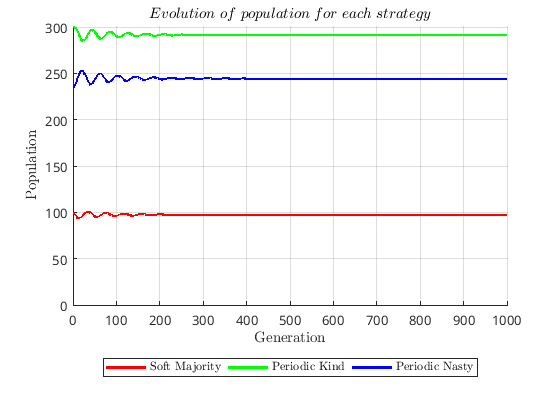
\includegraphics[width=\textwidth]{population_size_sensitivity_before_off.png}
        \caption{Before}
    \end{subfigure}
    \hfill
    \begin{subfigure}[t]{0.45\textwidth}
        \centering
        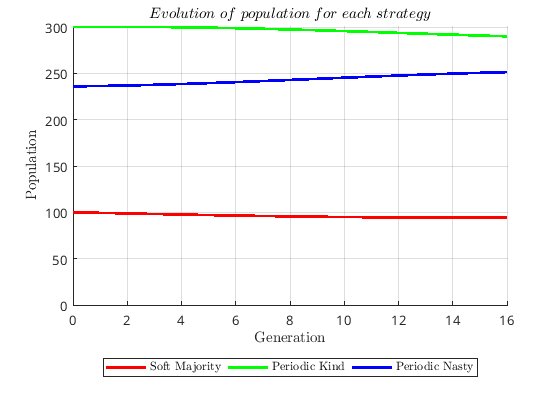
\includegraphics[width=\textwidth]{population_size_sensitivity_after_off.png}
        \caption{After}
    \end{subfigure}
    \caption{Side-by-side comparison of population size sensitivity before and after Off}
\end{figure}

\newpage
\subsection{Population size sensitivity 2}
This is an example of generally oscillatory behavior becoming eager to converge through either smoother oscillations or steady states. 
\begin{figure}[H]
    \centering
    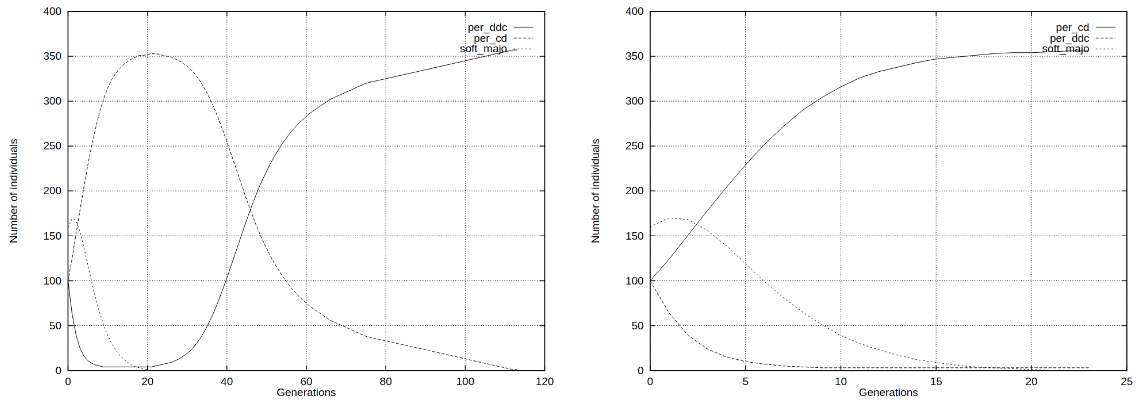
\includegraphics[width=0.8\textwidth]{population_size_sensitivity_2.png}
    \caption{Population size sensitivity 2 Original Plot}
\end{figure}
\begin{table}[H]
    \centering
    \begin{tabular}{|l|c|}
    \hline
    \textbf{Strategy}  & \textbf{Population} \\
    \hline
    soft\_majo   &  100 \\
    per\_ccd     &  300 \\
    per\_ddc    &  159 $\rightarrow$ 160 \\
    \hline
    \multicolumn{2}{|l|}{\textbf{Notes:}} \\
        \multicolumn{2}{|l|}{Rounds = 1000} \\
        \multicolumn{2}{|l|}{Generations = 120 $\rightarrow$ 50} \\
        \multicolumn{2}{|l|}{Matrix = \(\begin{bmatrix} 3 & 0 \\ 5 & 1 \end{bmatrix}\)} \\
    \hline
    \end{tabular}
    \caption{Initial populations}
\end{table}

\begin{figure}[H]
    \centering
    \begin{subfigure}[t]{0.45\textwidth}
        \centering
        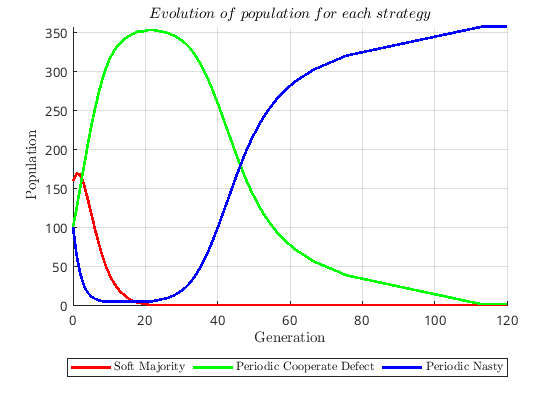
\includegraphics[width=\textwidth]{population_size_sensitivity_2_before_paper.png}
        \caption{Before}
    \end{subfigure}
    \hfill
    \begin{subfigure}[t]{0.45\textwidth}
        \centering
        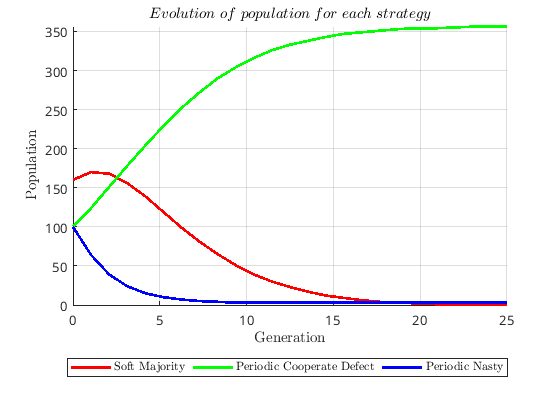
\includegraphics[width=\textwidth]{population_size_sensitivity_2_after_paper.png}
        \caption{After}
    \end{subfigure}
    \caption{Side-by-side comparison of population size sensitivity 2 before and after Paper method}
\end{figure}

\begin{figure}[H]
    \centering
    \begin{subfigure}[t]{0.45\textwidth}
        \centering
        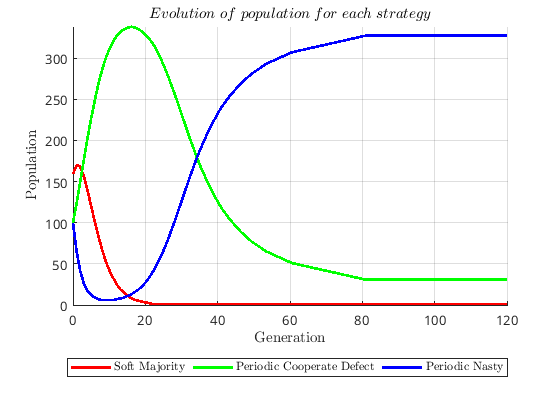
\includegraphics[width=\textwidth]{population_size_sensitivity_2_before_dec.png}
        \caption{Before}
    \end{subfigure}
    \hfill
    \begin{subfigure}[t]{0.45\textwidth}
        \centering
        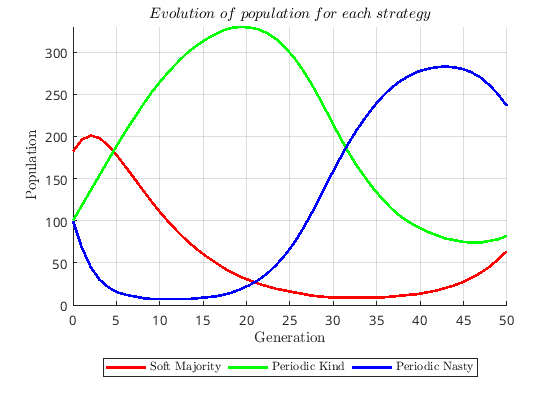
\includegraphics[width=\textwidth]{population_size_sensitivity_2_after_dec.png}
        \caption{After}
    \end{subfigure}
    \caption{Side-by-side comparison of population size sensitivity 2 before and after Dec method}
\end{figure}
\begin{figure}[H]
    \centering
    \begin{subfigure}[t]{0.45\textwidth}
        \centering
        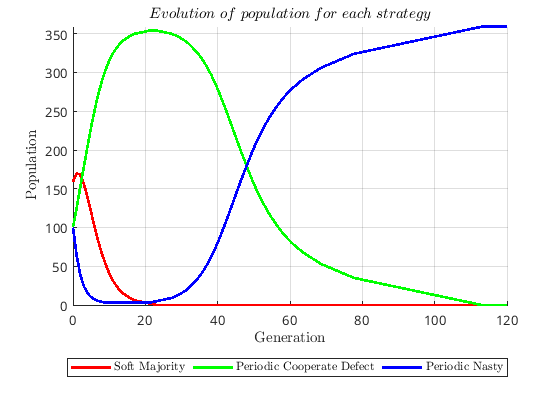
\includegraphics[width=\textwidth]{population_size_sensitivity_2_before_pop.png}
        \caption{Before}
    \end{subfigure}
    \hfill
    \begin{subfigure}[t]{0.45\textwidth}
        \centering
        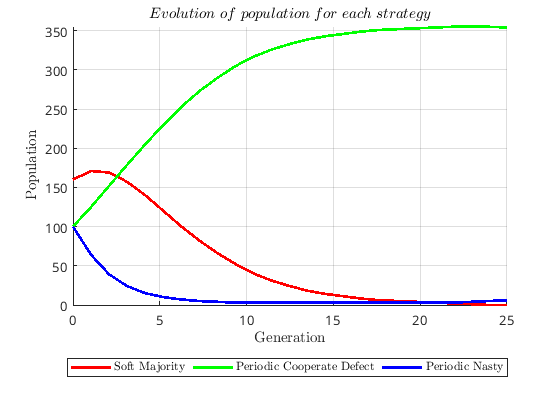
\includegraphics[width=\textwidth]{population_size_sensitivity_2_after_pop.png}
        \caption{After}
    \end{subfigure}
    \caption{Side-by-side comparison of population size sensitivity 2 before and after Pop method}
\end{figure}

\begin{figure}[H]
    \centering
    \begin{subfigure}[t]{0.45\textwidth}
        \centering
        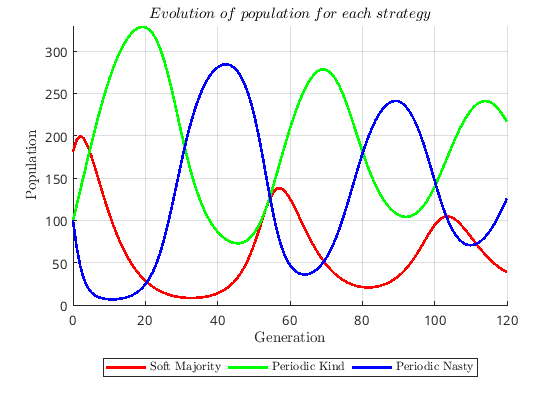
\includegraphics[width=\textwidth]{population_size_sensitivity_2_before_off.png}
        \caption{Before}
    \end{subfigure}
    \hfill
    \begin{subfigure}[t]{0.45\textwidth}
        \centering
        \includegraphics[width=\textwidth]{population_size_sensitivity_2_after_off.png}
        \caption{After}
    \end{subfigure}
    \caption{Side-by-side comparison of population size sensitivity 2 before and after Off method}
\end{figure}

\newpage
\subsection{Game length sensitivity}
This experiment examines the case of changing the game's length or the number of rounds played by the players each generation. In the before State the peaks reached are higher in the paper compared to our example, however we manage to capture the change in converging speed and amplitude of the oscillations. The rounding methods that recreate the general shape of the plot are "dec" and "off". In the case of "pop" we notice periodic oscillations of the after state, which do not decrease in amplitude.
\begin{figure}[H]
    \centering
    \includegraphics[width=0.8\textwidth]{game_length_sensitivity.png}
    \caption{Game length sensitivity Original Plot}
\end{figure}
\begin{table}[H]
    \centering
    \begin{tabular}{|l|c|}
        \hline
        \textbf{Strategy}  & \textbf{Population} \\
        \hline
        soft\_majo   &  100 \\
        per\_ccd     &  300 \\
        per\_ddc     &  244 \\
        \hline
        \multicolumn{2}{|l|}{\textbf{Notes:}} \\
        \multicolumn{2}{|l|}{Rounds = 6 $\rightarrow$ 7} \\
        \multicolumn{2}{|l|}{Generations = 1000 $\rightarrow$ 250} \\
        \multicolumn{2}{|l|}{Matrix = \(\begin{bmatrix} 3 & 0 \\ 5 & 1 \end{bmatrix}\)} \\
        \hline
    \end{tabular}
    \caption{Initial populations with additional notes}
\end{table}
\begin{figure}[H]
    \centering
    \begin{subfigure}[t]{0.45\textwidth}
        \centering
        \includegraphics[width=\textwidth]{game_length_sensitivity_before_paper.png}
        \caption{Before}
    \end{subfigure}
    \hfill
    \begin{subfigure}[t]{0.45\textwidth}
        \centering
        \includegraphics[width=\textwidth]{game_length_sensitivity_after_paper.png}
        \caption{After}
    \end{subfigure}
    \caption{Side-by-side comparison of game length sensitivity before and after Paper}
\end{figure}

\begin{figure}[H]
    \centering
    \begin{subfigure}[t]{0.45\textwidth}
        \centering
        \includegraphics[width=\textwidth]{game_length_sensitivity_before_dec.png}
        \caption{Before}
    \end{subfigure}
    \hfill
    \begin{subfigure}[t]{0.45\textwidth}
        \centering
        \includegraphics[width=\textwidth]{game_length_sensitivity_after_dec.png}
        \caption{After}
    \end{subfigure}
    \caption{Side-by-side comparison of game length sensitivity before and after Dec}
\end{figure}

\begin{figure}[H]
    \centering
    \begin{subfigure}[t]{0.45\textwidth}
        \centering
        \includegraphics[width=\textwidth]{game_length_sensitivity_before_pop.png}
        \caption{Before}
    \end{subfigure}
    \hfill
    \begin{subfigure}[t]{0.45\textwidth}
        \centering
        \includegraphics[width=\textwidth]{game_length_sensitivity_after_pop.png}
        \caption{After}
    \end{subfigure}
    \caption{Side-by-side comparison of game length sensitivity before and after Pop}
\end{figure}

\begin{figure}[H]
    \centering
    \begin{subfigure}[t]{0.45\textwidth}
        \centering
        \includegraphics[width=\textwidth]{game_length_sensitivity_before_off.png}
        \caption{Before}
    \end{subfigure}
    \hfill
    \begin{subfigure}[t]{0.45\textwidth}
        \centering
        \includegraphics[width=\textwidth]{game_length_sensitivity_after_off.png}
        \caption{After}
    \end{subfigure}
    \caption{Side-by-side comparison of game length sensitivity before and after Off}
\end{figure}

\newpage
\subsection{Payoff matrix sensitivity}
This meeting highlights the effects a slight change to one of the payoff matrix values can have on the results. In the before State we see increasing oscillations and after changing the defector's exploiting payoff these oscillations become periodic. We perfectly replicate the paper's results using all of our rounding methods. An interesting observation is that "pop" is reaching a final before State a lot quicker ($\approx$ 400 generations) than the other two methods ($\approx$ 1000 generations)
\begin{figure}[H]
    \centering
    \includegraphics[width=0.8\textwidth]{payoff_matrix_sensitivity.png}
    \caption{Payoff matrix sensitivity Original Plot}
\end{figure}
\begin{table}[H]
    \centering
    \begin{tabular}{|l|c|}
        \hline
        \textbf{Strategy}  & \textbf{Population} \\
        \hline
        soft\_majo   &  100 \\
        per\_ccd     &  300 \\
        per\_ddc     &  244 \\
        \hline
        \multicolumn{2}{|l|}{\textbf{Notes:}} \\
        \multicolumn{2}{|l|}{Rounds = 1000} \\
        \multicolumn{2}{|l|}{Generations = 500 $\rightarrow$ 1000} \\
        \multicolumn{2}{|l|}{Matrix = \(\begin{bmatrix} 3 & 0 \\ 4.6 \rightarrow 4.7 & 1 \end{bmatrix}\)} \\
        \hline
    \end{tabular}
    \caption{Initial populations with additional notes}
\end{table}
\begin{figure}[H]
    \centering
    \begin{subfigure}[t]{0.45\textwidth}
        \centering
        \includegraphics[width=\textwidth]{payoff_matrix_sensitivity_before_paper.png}
        \caption{Before}
    \end{subfigure}
    \hfill
    \begin{subfigure}[t]{0.45\textwidth}
        \centering
        \includegraphics[width=\textwidth]{payoff_matrix_sensitivity_after_paper.png}
        \caption{After}
    \end{subfigure}
    \caption{Side-by-side comparison of payoff matrix sensitivity before and after Paper}
\end{figure}

\begin{figure}[H]
    \centering
    \begin{subfigure}[t]{0.45\textwidth}
        \centering
        \includegraphics[width=\textwidth]{payoff_matrix_sensitivity_before_dec.png}
        \caption{Before}
    \end{subfigure}
    \hfill
    \begin{subfigure}[t]{0.45\textwidth}
        \centering
        \includegraphics[width=\textwidth]{payoff_matrix_sensitivity_after_dec.png}
        \caption{After}
    \end{subfigure}
    \caption{Side-by-side comparison of payoff matrix sensitivity before and after Dec}
\end{figure}

\begin{figure}[H]
    \centering
    \begin{subfigure}[t]{0.45\textwidth}
        \centering
        \includegraphics[width=\textwidth]{payoff_matrix_sensitivity_before_pop.png}
        \caption{Before}
    \end{subfigure}
    \hfill
    \begin{subfigure}[t]{0.45\textwidth}
        \centering
        \includegraphics[width=\textwidth]{payoff_matrix_sensitivity_after_pop.png}
        \caption{After}
    \end{subfigure}
    \caption{Side-by-side comparison of payoff matrix sensitivity before and after Pop}
\end{figure}

\begin{figure}[H]
    \centering
    \begin{subfigure}[t]{0.45\textwidth}
        \centering
        \includegraphics[width=\textwidth]{payoff_matrix_sensitivity_before_off.png}
        \caption{Before}
    \end{subfigure}
    \hfill
    \begin{subfigure}[t]{0.45\textwidth}
        \centering
        \includegraphics[width=\textwidth]{payoff_matrix_sensitivity_after_off.png}
        \caption{After}
    \end{subfigure}
    \caption{Side-by-side comparison of payoff matrix sensitivity before and after Off}
\end{figure}

\subsection{Rounding method sensitivity}
The final category of minor changes leading to different results is the rounding method. Though out the meetings analysis we have highlighted the importance of the rounding method since to replicate the paper's results we resorted to creating more than one methods, alternating between all of them to better illustrate the effects mentioned in the paper. On the first example we see periodic movements become attenuated oscillations and ultimately steady states. The rounding method used in the before state is "dec", "pop" and in the after state it is "off" or no rounding.
\begin{figure}[H]
    \centering
    \includegraphics[width=0.8\textwidth]{rounding_method_sensitivity.png}
    \caption{Rounding method sensitivity Original Plot}
\end{figure}
\begin{table}[H]
    \centering
    \begin{tabular}{|l|c|}
        \hline
        \textbf{Strategy}  & \textbf{Population} \\
        \hline
        soft\_majo   &  100 \\
        per\_ccd     &  300 \\
        per\_ddc     &  200 \\
        \hline
        \multicolumn{2}{|l|}{\textbf{Notes:}} \\
        \multicolumn{2}{|l|}{Rounds = 1000} \\
        \multicolumn{2}{|l|}{Generations = 1000} \\
        \multicolumn{2}{|l|}{Matrix = \(\begin{bmatrix} 3 & 0 \\ 5 & 1 \end{bmatrix}\)} \\
        \hline
    \end{tabular}
    \caption{Initial populations with additional notes}
\end{table}
\begin{figure}[H]
    \centering
    \begin{subfigure}[t]{0.45\textwidth}
        \centering
        \includegraphics[width=\textwidth]{rounding_method_sensitivity_before_paper.png}
        \caption{Before}
    \end{subfigure}
    \hfill
    \begin{subfigure}[t]{0.45\textwidth}
        \centering
        \includegraphics[width=\textwidth]{rounding_method_sensitivity_after_off.png}
        \caption{After}
    \end{subfigure}
    \caption{Side-by-side comparison of rounding method sensitivity before (Paper) and after (Off)}
\end{figure}
\begin{figure}[H]
 \begin{subfigure}[t]{0.45\textwidth}
        \centering
        \includegraphics[width=\textwidth]{rounding_method_sensitivity_before_dec.png}
        \caption{Before}
    \end{subfigure}
    \hfill
    \begin{subfigure}[t]{0.45\textwidth}
        \centering
        \includegraphics[width=\textwidth]{rounding_method_sensitivity_after_off.png}
        \caption{After}
    \end{subfigure}
    \caption{Side-by-side comparison of rounding method sensitivity before (Dec) and after (Off)}
\end{figure}

\begin{figure}[H]
 \begin{subfigure}[t]{0.45\textwidth}
        \centering
        \includegraphics[width=\textwidth]{rounding_method_sensitivity_before_pop.png}
        \caption{Before}
    \end{subfigure}
    \hfill
    \begin{subfigure}[t]{0.45\textwidth}
        \centering
        \includegraphics[width=\textwidth]{rounding_method_sensitivity_after_off.png}
        \caption{After}
    \end{subfigure}
    \caption{Side-by-side comparison of rounding method sensitivity before (Pop) and after (Off)}
\end{figure}

\newpage
\subsection{Rounding method sensitivity 2}
The second example is best displayed using the "pop" method. Here we divide our initial populations by ten making rounding more important since we round an substantially larger section of the individual populations. The "off" and "dec" methods do not display the same behavior on the after state but rather they seem to be a micrography of the before state. 
\begin{figure}[H]
    \centering
    \includegraphics[width=0.8\textwidth]{rounding_method_sensitivity_2.png}
    \caption{Rounding method sensitivity 2 Original Plot}
\end{figure}
\begin{table}[H]
    \centering
    \begin{tabular}{|l|c|}
        \hline
        \textbf{Strategy}  & \textbf{Population} \\
        \hline
        soft\_majo   &  100 $\rightarrow$ 10 \\
        per\_ccd     &  450 $\rightarrow$ 45 \\
        per\_ddc     &  1000 $\rightarrow$ 100\\
        \hline
        \multicolumn{2}{|l|}{\textbf{Notes:}} \\
        \multicolumn{2}{|l|}{Rounds = 1000} \\
        \multicolumn{2}{|l|}{Generations = 450 $\rightarrow$ 160} \\
        \multicolumn{2}{|l|}{Matrix = \(\begin{bmatrix} 3 & 0 \\ 5 & 1 \end{bmatrix}\)} \\
        \hline
    \end{tabular}
    \caption{Initial populations with additional notes}
\end{table}
\begin{figure}[H]
    \centering
    \begin{subfigure}[t]{0.45\textwidth}
        \centering
        \includegraphics[width=\textwidth]{rounding_method_sensitivity_2_before_paper.png}
        \caption{Before}
    \end{subfigure}
    \hfill
    \begin{subfigure}[t]{0.45\textwidth}
        \centering
        \includegraphics[width=\textwidth]{rounding_method_sensitivity_2_after_paper.png}
        \caption{After}
    \end{subfigure}
    \caption{Side-by-side comparison of rounding method sensitivity 2 before and after Paper}
\end{figure}

\begin{figure}[H]
    \centering
    \begin{subfigure}[t]{0.45\textwidth}
        \centering
        \includegraphics[width=\textwidth]{rounding_method_sensitivity_2_before_pop.png}
        \caption{Before}
    \end{subfigure}
    \hfill
    \begin{subfigure}[t]{0.45\textwidth}
        \centering
        \includegraphics[width=\textwidth]{rounding_method_sensitivity_2_after_pop.png}
        \caption{After}
    \end{subfigure}
    \caption{Side-by-side comparison of rounding method sensitivity 2 before and after Pop}
\end{figure}

\begin{figure}[H]
    \centering
    \begin{subfigure}[t]{0.45\textwidth}
        \centering
        \includegraphics[width=\textwidth]{rounding_method_sensitivity_2_before_dec.png}
        \caption{Before}
    \end{subfigure}
    \hfill
    \begin{subfigure}[t]{0.45\textwidth}
        \centering
        \includegraphics[width=\textwidth]{rounding_method_sensitivity_2_after_dec.png}
        \caption{After}
    \end{subfigure}
    \caption{Side-by-side comparison of rounding method sensitivity 2 before and after Dec}
\end{figure}

\begin{figure}[H]
    \centering
    \begin{subfigure}[t]{0.45\textwidth}
        \centering
        \includegraphics[width=\textwidth]{rounding_method_sensitivity_2_before_off.png}
        \caption{Before}
    \end{subfigure}
    \hfill
    \begin{subfigure}[t]{0.45\textwidth}
        \centering
        \includegraphics[width=\textwidth]{rounding_method_sensitivity_2_after_off.png}
        \caption{After}
    \end{subfigure}
    \caption{Side-by-side comparison of rounding method sensitivity 2 before and after Off}
\end{figure}


\chapter{Imitation Dynamics}
\section{Imitation dynamics}

In imitation dynamics, after a meeting among players adopting different strategies is concluded, a number of players adopt (imitate) one of the best performing strategies of the previous generation. The best performing strategies are those that received the highest payoff in the previous generation and we can have more than one of them. A strategy's payoff depends, not only on the specific strategies competing, but also on the proportion of players representing the strategy in a generation.
\\\\
In what follows, we will restrict ourselves to three competing strategies with the total population of $N$ players kept constant from generation to generation. We will also consider that after a meeting is concluded, a single player is chosen randomly, from the strategies that have non zero populations and that this player chooses randomly, with equal probability, to adopt one of the strategies that scored the most in that previous meeting.
\\\\
The state of the system can be represented in this case by a triplet $(n_1,n_2,n_3)$ of the players adopting each one of the three strategies, with $n_i \in \mathbb{Z},\ \ 0 \leq n_i \leq N,\ \ n_1+n_2+n_3=N$. The evolution of the state through the different generations (extending the evolutionary game to run for an infinite number of steps), is a Markov chain. This Markov chain has in general a non deterministic state transition matrix M, due to the probabilistic adoption of one of the best strategies, by one player, at the end of a generation. In the sequel we will calculate theoretically and by simulation, this state transition matrix.

\subsection{Theoretical approach}

In order to calculate theoretically the state transition matrix M, one needs the population of each one of the three strategies at the beginning of a generation, the total payoff of each strategy during a meeting  and the rules for transition from one state to the possible next states. For the transition rules, it suffices to know the strategies from which a player can leave, and the best scoring strategies in the meeting and then easily calculate the probabilities of transition for all the possibly adopted new strategies.
\\\\
The total payoff of each strategy during a meeting equals the sum of the scores that individual players following that strategy can gain, during all two-by-two games in the two-by-two round robin tournament. Consequently, it suffices to calculate the score of each player during a match between two players. This can of course be achieved by simulation, but also, for certain deterministic strategies this can be evaluated without simulating a match. For example, during an All-C vs All-D match, the players choose C and D, respectively at each round, and the All-C player's match score is SU, while the All-D player's match score is TU, with
\begin{center}
 \begin{tabular}{|c|c|c|c|}
\hline
 & $C$ & $D$ \\
 \hline
$C$ & \begin{tabular}{c}
R\\
R
\end{tabular} &\begin{tabular}{c}
S\\
T
\end{tabular} \\
\hline
$D$ &  \begin{tabular}{c}
T\\
S
\end{tabular}  &  \begin{tabular}{c}
P\\
P
\end{tabular}  \\
\hline
\end{tabular} 
\end{center}
the payoff matrix and U the number of rounds per game. $R$ is the Reward payoff, $P$ the Punishment payoff, $T$ the Temptation payoff and $S$ the Sucker's payoff. $T>R>P>S$ guarantees that the Nash equilibrium is mutual defection, whereas $2R>T+S$ makes mutual cooperation the globally best outcome. However, this road of investigation cannot be extended to more involved strategies and certainly is not adequate for probabilistic strategies. Thereof, instead of calculating the exact score a player can gain during a match, either by simulation, or as a deterministic function of game histories in simple cases, we can instead use the expected average payoff, per round, of each player.
\\\\
The expected average payoff per round can be calculated by using the fact that a match between two players can also be modeled as a finite-state Markov chain, where the system transits among the four states CC, CD, DC, DD. By adopting  this method, we can extend the calculation of the state transition matrix even in the case of probabilistic strategies, like the zero determinant and extortionate strategies that will be presented hereafter.








\subsubsection{Computation of expected average payoff per round, using Markov chains}\label{expected}
In one round of the match, the outcome can be CC, CD, DC, or DD, where C = cooperation and D = defection. In each pair, the first letter represents the choice of the first player and the second the choice of the second player. In games where both players adopt strategies based on memory of the previous round (memory-one strategies), but also more generally in the case of finite-memory strategies, a match can be modeled as a finite-state Markov chain, where the system transitions between the four states CC, CD, DC, DD \cite{hillier2020}. The conditional probabilities of any future event depend only on the current state and are independent of any past event.

Thus, the one-step transition matrix \( M \) has the form:
\[
M =
\begin{bmatrix}
p(\text{CC}|\text{CC}) & p(\text{CC}|\text{CD}) & p(\text{CC}|\text{DC}) & p(\text{CC}|\text{DD}) \\
p(\text{CD}|\text{CC}) & p(\text{CD}|\text{CD}) & p(\text{CD}|\text{DC}) & p(\text{CD}|\text{DD}) \\
p(\text{DC}|\text{CC}) & p(\text{DC}|\text{CD}) & p(\text{DC}|\text{DC}) & p(\text{DC}|\text{DD}) \\
p(\text{DD}|\text{CC}) & p(\text{DD}|\text{CD}) & p(\text{DD}|\text{DC}) & p(\text{DD}|\text{DD})
\end{bmatrix}
\]
For example, \( p(\text{CD}|\text{DC}) = p(X_{k+1} = \text{CD} | X_k = \text{DC}) \) is the probability that the next state is CD, given that the current state is DC (the first player chooses C and the second D, while their previous moves were D and C, respectively).

Assuming independence of the players' choices:
\[
p(\text{CD}|\text{DC}) = p_X(C|\text{DC}) \cdot p_Y(D|\text{DC}) = p_X(C|\text{DC}) \cdot (1 - p_Y(C|\text{DC}))
\]
where \[
 p_X(C|\text{DC}) 
\]
is the probability that the first player chooses C for his next move, when the previous state was DC, and 
\[
 p_Y(D|\text{DC}) 
\]
is the probability that the second player chooses D for his next move, when the previous state was DC. It is important to be able to calculate these conditional probabilities: \[
p_X(C|\text{CC}) ,p_X(C|\text{CD}), p_X(C|\text{DC}), p_X(C|\text{DD}) 
\]
that is, the probabilities for a player to choose C given that the previous state was CC, or CD, or DC, or DD, which are dependent on the specific strategy that the player has adopted.

Let us define:

\[
\mathbf{p} = (p_1, p_2, p_3, p_4) = (p_X(C|\text{CC}), p_X(C|\text{CD}), p_X(C|\text{DC}), p_X(C|\text{DD}))
\]
\[
\mathbf{q} = (q_1, q_2, q_3, q_4) = (p_Y(C|\text{CC}), p_Y(C|\text{CD}), p_Y(C|\text{DC}), p_Y(C|\text{DD}))
\]
the strategy vectors for the first player, and the second player, respectively. The strategy vector $\mathbf{p}$ can be calculated for each strategy.
For example:
\begin{itemize}
  \item Random strategy: \( \mathbf{p} = (0.5, 0.5, 0.5, 0.5) \)
  \item All-C: \( \mathbf{p} = (1, 1, 1, 1) \)
  \item All-D: \( \mathbf{p} = (0, 0, 0, 0) \)
  \item Tit-For-Tat: \( \mathbf{p} = (1, 0, 1, 0) \)
  \item Generous Tit-For-Tat (GTFT): \( \mathbf{p} = (1, q, 1, q) \), since, in comparison with Tit-for-Tat, when the opponent has played D, GTFT responds with D with a probability of $1-q$
  \item Pavlov (Win State Lose Shift): \( \mathbf{p} = (1, 0, 0, 1) \)
\end{itemize}

Using these vectors, the one-step transition matrix \( M \) becomes:

\[
M =
\begin{bmatrix}
p_1 q_1 & p_1 (1 - q_1) & (1 - p_1) q_1 & (1 - p_1)(1 - q_1) \\
p_2 q_3 & p_2 (1 - q_3) & (1 - p_2) q_3 & (1 - p_2)(1 - q_3) \\
p_3 q_2 & p_3 (1 - q_2) & (1 - p_3) q_2 & (1 - p_3)(1 - q_2) \\
p_4 q_4 & p_4 (1 - q_4) & (1 - p_4) q_4 & (1 - p_4)(1 - q_4)
\end{bmatrix}
\]
Each row of \( M \) must sum to 1. Let it be noted that in the second row, the system transits to a CD state (given the current state CC, CD, DC, DD) and thus the second player transits to a D state. For that reason, \(
q_3 = p_Y(C|\text{DC}) 
\), which represents the probability that the second player chooses C, given the previous state was DC and not  \(
q_2 
\)  is used. Similar observations can be made about the third row.
\\\\
It is also important to be able to calculate the unconditional (marginal) probabilities that the system will be driven in a CC, CD, DC or DD state, and how these are evolving through generations. 
Let \( v_k \) be the vector of unconditional probabilities at step \( k \):
\[
v_k = \begin{bmatrix}
p(X_k = \text{CC}) ,  p(X_k = \text{CD}) ,  p(X_k = \text{DC}) ,  p(X_k = \text{DD})
\end{bmatrix}
\]

Then, using the law of total probability: \[
\begin{aligned}
p(X_{k+1} = CD) &= p(X_{k+1} = CD \mid X_k = CC) \, p(X_k = CC) \\
&\quad + p(X_{k+1} = CD \mid X_k = CD) \, p(X_k = CD) \\
&\quad + p(X_{k+1} = CD \mid X_k = DC) \, p(X_k = DC) \\
&\quad + p(X_{k+1} = CD \mid X_k = DD) \, p(X_k = DD) \\
&= 
\begin{bmatrix}
p(CD \mid CC) , p(CD \mid CD) , p(CD \mid DC) , p(CD \mid DD)
\end{bmatrix}
\cdot
\begin{bmatrix}
p(X_k = CC) \\
p(X_k = CD) \\
p(X_k = DC) \\
p(X_k = DD)
\end{bmatrix}
\end{aligned}
\]

In conclusion, in the last equation where we used the simpler notation adopted in the transition matrix \( M \), we have that \( p(X_{k+1} = CD) \), which is an element of the vector \( v_{k+1} \), equals the inner product of the second row of the one-step transition matrix \( M \) and the vector \( v_k \). Therefore, overall, the temporal evolution of \( v_k \) follows \( v_{k+1} = M v_k \), and recursively \( v_{k+1} = M^{k+1} v_0 \), where \( v_0 \) is the vector of unconditional probabilities for the system to be in one of the states \( CC, CD, DC, DD \) at the step when the players make their initial moves.  Thus, the matrix \( M^m \) is the matrix of conditional probabilities over \( m \) steps (the \( m \)-step transition matrix), and includes all the conditional probabilities for transitioning from any current state \( CC, CD, DC, DD \) to any other state \( CC, CD, DC, DD \) in \( m \) steps of the game (Chapman-Kolmogorov equations).


It is proven that when the Markov chain is irreducible and ergodic, the vector \( v_k \) of unconditional probabilities converges \( (\lim_{k \to \infty} v_k = \pi) \) to the stationary distribution \( \pi \), which is also given by the convergent limit 

\[
\pi = \lim_{n \to \infty} \frac{1}{n} \sum_{k=0}^{n-1} v_0 M^k
\]

When this limit exists, it is independent of \( v_0 \). Clearly, for \( \pi \), it holds that \( \pi M = \pi \) (obtained from the relation \( v_{k+1} = M v_k \) in the limit \( k \to \infty \)), and the sum of the elements of \( \pi \) is equal to 1, as it represents the unconditional probabilities, in the steady state, that the system is found in one of the states \( CC, CD, DC, DD \). 

Then, the elements of each column of the matrix \( M^m \), for large \( m \), approach the same value, since the conditional probability of transitioning to a state in \( m \) steps for large \( m \) becomes independent of the current state of the system. Knowing now, for a game between two opponents \( X \) and \( Y \), the vector \( \pi \) with the long-term probabilities of the system being in any of the states \( CC, CD, DC, DD \), it is clear that we can calculate the average expected pay-off per round for each of the two opponents, using the formulas:

\[
s_X = \pi S_X = \pi
\begin{bmatrix}
R \\
S \\
T \\
P
\end{bmatrix}
\quad \text{and} \quad
s_Y = \pi S_Y = \pi
\begin{bmatrix}
R \\
T \\
S \\
P
\end{bmatrix}
\]

respectively.
\subsubsection{Theoretical calculation of the state transition matrix using Markov chains}\label{Theo calc}
In the sequel, we will consider a tournament between $M=3$ strategies with an imitating behavior, let us call them $A,\ B$ and $C$, with $n_1,\ n_2$ and $n_3$ being their respective population at a certain generation. During all generations, the total population remains constant at $N=n_1+n_2+n_3$. At each generation, we consider a two-by-two round robin tournament between all the players, where each player of strategy $X$ plays a number of games with opponents $Y$ of his strategy group, or with opponents from the other strategies, according to the table given hereafter:
\\\\
\begin{center}
    

\begin{tabular}{|c|c|c|c|}
 \hline
 \diagbox{$X$}{$Y$} & $A$ & $B$ & $C$ \\ 
 \hline
$A$ & $\frac{n_1(n_1-1)}{2}$ & $n_1n_2$ & $n_1n_3$ \\
 \hline
$B$ &  & $\frac{n_2(n_2-1)}{2}$ & $n_2n_3$ \\
 \hline
$C$ &  &  & $\frac{n_3(n_3-1)}{2}$ \\
 \hline
\end{tabular}

\end{center}

From our previous analysis, considering the Markov chain of a certain game between two players, having as states all the possible outcomes of the game $(CC, \ \ CD, \ \ DC, \ \ DD)$, we were able to calculate the mean expected payoff for each one of the two players. More precisely, having the strategy vectors $$\mathbf{p}=(p_X(C|CC)\ \ p_X(C|CD)\ \ p_X(C|DC)\ \ p_X(C|DD))$$ and $$\mathbf{q}=(p_Y(C|CC)\ \ p_Y(C|CD)\ \ p_Y(C|DC)\ \ p_Y(C|DD))$$ we can calculate the one-step transition matrix $M(\mathbf{p}, \mathbf{q})$, then the stationary distribution $\pi$ from $\pi M=\pi$ and $\sum_{i}\pi(i)=1$ and finally the expected average payoff per round for each one of the two players as 
$$s_X=\pi S_X=\pi
\begin{bmatrix}
R \\
S \\
T \\
P 
\end{bmatrix}\ ,
s_Y=\pi S_Y=\pi
 \begin{bmatrix}
R \\
T \\
S \\
P 
\end{bmatrix}$$

with

\begin{center}
 \begin{tabular}{|c|c|c|c|}
\hline
 & $C$ & $D$ \\
 \hline
$C$ & \begin{tabular}{c}
R\\
R
\end{tabular} &\begin{tabular}{c}
S\\
T
\end{tabular} \\
\hline
$D$ &  \begin{tabular}{c}
T\\
S
\end{tabular}  &  \begin{tabular}{c}
P\\
P
\end{tabular}  \\
\hline
\end{tabular} 
\end{center}
the game payoff matrix.
In a meeting (tournament) of 3 strategies, let us denote with
$$\mathbf{P}=[P_{AA}^A,\ \ P_{BB}^B,\ \ P_{CC}^C,\ \ P_{AB}^A,\ \ P_{AB}^B,\ \ P_{AC}^A,\ \ P_{AC}^C,\ \ P_{BC}^B,\ \ P_{BC}^C]$$
a vector comprising all the payoffs between two players. In $\mathbf{P}$, $P_{XY}^X$ denotes the payoff for player $X$ in a match between $X$ and $Y$ and $P_{XY}^Y$ the payoff of player $Y$ in the same match. Obviously, considering all the matches in a meeting, if each match comprises $U$ rounds, the total expected average payoff for each one of the three strategies is given by
$$\text{strategy A:} \ \ SC_A=[n_1(n_1-1)P_{AA}^A+n_1n_2P_{AB}^A+n_1n_3P_{AC}^A]U$$

$$\text{strategy B:} \ \ SC_B=[n_1n_2P_{AB}^B+n_2(n_2-1)P_{BB}^B+n_2n_3P_{BC}^B]U$$

$$\text{strategy C:} \ \ SC_C=[n_1n_3P_{AC}^C+n_2n_3P_{BC}^C+n_3(n_3-1)P_{CC}^C]U$$
Note here that in a match between two players of the same strategy, the strategy payoff is $2P_{XX}^X$. We are now ready, for the specific choice of strategies $A, B$ and $C$ and for all combinations of populations $n_1,\ n_2,\ n_3$, such that $n_1+n_2+n_3=N$, $n_i\in \mathbb{Z}$, $0\le n_i\le N$, to calculate the total expected average payoffs for the three strategies $(SC_A,\ SC_B ,\ SC_C)$ and find which can be the next state. In general, being at a certain state $(n_1, \ n_2,\ n_3)$, the next state can be one of the following: $(n_1,\ n_2,\ n_3)$, or $(n_1+1,\ n_2-1,\ n_3)$, or $(n_1+1,\ n_2,\ n_3-1)$, or $(n_1-1,\ n_2+1,\ n_3)$, or $(n_1,\ n_2+1,\ n_3-1)$, or $(n_1-1,\ n_2,\ n_3+1)$, or $(n_1,\ n_2-1,\ n_3+1)$, as far as $n_1\pm1,\ n_2\pm1,\ n_3\pm1$ remain integers in the region $[0,N]$.
\\\\
After ordering the three strategies in descending order, based on their scores ${SC}_A$, ${SC}_B$, ${SC}_C$ in a meeting, and supposing that the strategies have $n_1$, $n_2$, $n_3$ players respectively in the current state, we have the following mutually independent cases for the movements of a player from a state to another one, together with their respective probabilities.

\begin{center}
\begin{tabular}{|c|c|c|c|}
\hline
\begin{tabular}{c}
Relations between scores  
\end{tabular}
& Current state & Next state & Probability \\ 
\hline
Rule 00: $SC_A$, $SC_B=$ $SC_C=0$ & $(n_1,\ \ 0,\ \ 0)$ & $(n_1,\ \ 0,\ \ 0)$ & $1$ \\
\hline
Rule 01: $SC_A>$ $SC_B,$ $SC_C=0$ & $(n_1,\ \ n_2,\ \ 0)$ & $(n_1+1,\ \ n_2-1,\ \ 0)$ & $\frac{n_2}{n_1+n_2}$ \\
&  & $(n_1,\ \ n_2,\ \ n_3)$ & $\frac{n_1}{n_1+n_2}$ \\
\hline
Rule 02: $SC_A=$ $SC_B,$ $SC_C=0$ & $(n_1,\ \ n_2,\ \ 0)$ & $(n_1,\ \ n_2,\ \ 0)$ & $\frac{1}{2}$ \\
&  & $(n_1+1,\ \ n_2-1,\ \ 0)$ & $\frac{1}{2}\frac{n_2}{n_1+n_2}$ \\
&  & $(n_1-1,\ \ n_2+1,\ \ 0)$ & $\frac{1}{2}\frac{n_1}{n_1+n_2}$ \\
\hline
Rule 03: $SC_A>$ $SC_B>$ $SC_C$ & $(n_1,\ \ n_2,\ \ n_3)$ & $(n_1,\ \ n_2,\ \ n_3)$ & $\frac{n_1}{n_1+n_2+n_3}$ \\
&  & $(n_1+1,\ \ n_2-1,\ \ n_3)$ & $\frac{n_2}{n_1+n_2+n_3}$ \\
&  & $(n_1+1,\ \ n_2,\ \ n_3-1)$ & $\frac{n_3}{n_1+n_2+n_3}$ \\
\hline
Rule 04: $SC_A=$ $SC_B>$ $SC_C$ & $(n_1,\ \ n_2,\ \ n_3)$ & $(n_1,\ \ n_2,\ \ n_3)$ & $\frac{1}{2}\frac{n_1+n_2}{n_1+n_2+n_3}$ \\
&  & $(n_1+1,\ \ n_2-1,\ \ n_3)$ & $\frac{1}{2}\frac{n_2}{n_1+n_2+n_3}$ \\
&  & $(n_1-1,\ \ n_2+1,\ \ n_3)$ & $\frac{1}{2}\frac{n_1}{n_1+n_2+n_3}$ \\
&  & $(n_1+1,\ \ n_2,\ \ n_3-1)$ & $\frac{1}{2}\frac{n_3}{n_1+n_2+n_3}$ \\
&  & $(n_1,\ \ n_2+1,\ \ n_3-1)$ & $\frac{1}{2}\frac{n_3}{n_1+n_2+n_3}$ \\
\hline
\begin{tabular}{c}
Rule 05: $SC_A>$ $SC_B=$ $SC_C$\\
(can be incorporated in rule 03)\\
\end{tabular}
& $(n_1,\ \ n_2,\ \ n_3)$ & $(n_1,\ \ n_2,\ \ n_3)$ & $\frac{n_1}{n_1+n_2+n_3}$ \\
&  & $(n_1+1,\ \ n_2-1,\ \ n_3)$ & $\frac{n_2}{n_1+n_2+n_3}$ \\
&  & $(n_1+1,\ \ n_2,\ \ n_3-1)$ & $\frac{n_3}{n_1+n_2+n_3}$ \\
\hline
Rule 06: $SC_A=$ $SC_B=$ $SC_C$ & $(n_1,\ \ n_2,\ \ n_3)$ & $(n_1,\ \ n_2,\ \ n_3)$ & $\frac{1}{3}$ \\
&  & $(n_1+1,\ \ n_2-1,\ \ n_3)$ & $\frac{1}{3}\frac{n_2}{n_1+n_2+n_3}$ \\
&  & $(n_1+1,\ \ n_2,\ \ n_3-1)$ & $\frac{1}{3}\frac{n_3}{n_1+n_2+n_3}$ \\
&  & $(n_1-1,\ \ n_2+1,\ \ n_3)$ & $\frac{1}{3}\frac{n_1}{n_1+n_2+n_3}$ \\
&  & $(n_1,\ \ n_2+1,\ \ n_3-1)$ & $\frac{1}{3}\frac{n_3}{n_1+n_2+n_3}$ \\
&  & $(n_1-1,\ \ n_2,\ \ n_3+1)$ & $\frac{1}{3}\frac{n_1}{n_1+n_2+n_3}$ \\
&  & $(n_1,\ \ n_2-1,\ \ n_3+1)$ & $\frac{1}{3}\frac{n_2}{n_1+n_2+n_3}$ \\
\hline
\end{tabular}
\end{center}
In the table above, we have supposed that a player is chosen randomly from the strategies which have non zero populations in the meeting and chooses randomly, with equal probability, to move to one of the strategies that scored the most in the meeting (more than one, if they draw).
\\
For example, in the case $SC_A=SC_B=SC_C$ (Rule 06) the three strategies have equal total expected average payoffs, a player can be chosen randomly from anyone of the strategies and move to anyone of the strategies. More precisely, we can remain in the same state $(n_1,n_2,n_3)$ if, either a player is chosen randomly from strategy $A$ with probability $\frac{n_1}{n_1+n_2+n_3}$ and moves to the same strategy $A$ with probability $\frac{1}{3}$, or a player is chosen from strategy $B$ and remains to $B$ with probability $\frac{1}{3}\frac{n_2}{_1+n_2+n_3}$, or a player is chosen from strategy $C$ and remains to $C$ with probability $\frac{1}{3}\frac{n_3}{n_1+n_2+n_3}$, all the probabilities summing to $\frac{1}{3}$. In an analogous manner, we have calculated all the reported state transitions in the table with their respective probabilities. Note that Rule 05 can be incorporated in Rule 03.
\\\\
Now that we can have the payoffs $P_{XY}^X,\ \ P_{XY}^Y$ for all combinations of strategies in a meeting, we can, for each combination of possible strategy populations (integers $n_1,\ n_2,\ n_3$ such that $\sum_{i}n_i=N, n_i\in \mathbb{Z},\ \ n_i\in [0,N]$), calculate the expected average payoffs $SC_A,\ SC_B,\ SC_C$ for each strategy and then apply the appropriate rule to obtain the next states to which the current state can transition, with the respective probabilities, thus obtaining the state transition matrix. We can provide all possible combinations by changing $n_1$ from $0$ to $N$, then for each $n_1$ changing $n_2$ from $0$ to $N-n_1$ and obtaining for each combination of $n_1, \ \ n_2$ the respective $n_3$ from $n_3=N-n_1-n_2$. There is a total of $(N+1)+N+(N-1)+...+2+1=\frac{((N+1)+1)(N+1)}{2}=\frac{(N+1)(N+2)}{2}$ combinations.

\subsubsection{Zero determinant and extortionate strategies}
For the three strategy meetings, we can choose between the well known strategies All-C, All-D, Random, Pavlov, Tit-for-Tat and Generous Tit-for-Tat. For these strategies we can easily calculate their strategy vector $\mathbf{p}$. Moreover, we can choose among some strategies which are called zero determinant strategies \cite{pressdyson2012} \cite{ncategory} \cite{wolfram}.
\\\\
A player using such a strategy, can enforce a linear relation $\alpha s_X+\beta s_Y+\gamma=0$, or $(s_X-P)=\chi(s_Y-P), \ \ \chi\ge 1$ between his score $s_X$ and his opponent's score $s_Y$. These strategies are based on the fact that it can be proven that, the inner product of a game's stationary distribution $\pi$ and an arbitrary $4\times 1$ vector $\mathbf{f}=[f_1,\ \ f_2,\ \ f_3,\ \ f_4]^T$ equals the determinant of a matrix:
\\\\
$\pi \cdot \mathbf{f}=\det\Big($
$
 \begin{bmatrix}
-1+p_1q_1 & -1+p_1 & -1+q_1 & f_1 \\
p_2q_3 & -1+p_2 & q_3 & f_2 \\
p_3q_2 & p_3 & -1+q_2 & f_3 \\
p_4q_4 & p_4 & q_4 & f_4 
\end{bmatrix} 
\Big)
$
$=\det[\overline{\mathbf{r}}(\mathbf{p},\mathbf{q})\ \ \tilde{\mathbf{p}}(\mathbf{p})\ \ \tilde{\mathbf{q}}(\mathbf{q})\ \ \mathbf{f}]$ with $\mathbf{p}=(p_1,\ \ p_2,\ \ p_3,\ \ p_4)$ and $\mathbf{q}=(q_1,\ \ q_2,\ \ q_3,\ \ q_4)$ the two strategy vectors.
\\\\
Notice here that the second column $\tilde{\mathbf{p}}$ of the matrix is solely under the control of $X$ while the third column $\tilde{\mathbf{q}}$ is solely under the control of $Y$, because they depend on $\mathbf{p}$ and $\mathbf{q}$, respectively, which $X$ and $Y$, respectively, can choose at their will. Player $X$ can choose $\mathbf{p}$ such that $\tilde{\mathbf{\mathbf{p}}}$ becomes equal to $\mathbf{f}$, subsequently zeroing the determinant and obtaining $\pi\cdot \mathbf{f}=0$ (hence the name zero determinant). By choosing $\mathbf{f}=\alpha S_X+\beta S_Y+\gamma\mathbf{1}$ with $\mathbf{1}=[1\ \ 1\ \ 1\ \ 1]^T$, it can be proven that $\alpha s_X+\beta s_Y+\gamma=0$, while by choosing $\mathbf{f}=(S_X-P\mathbf{1})-\chi(S_Y-P\mathbf{1})$ it can be proven that $(s_X-P)=\chi(s_Y-P)$.
\\\\
In the case $\alpha s_X+\beta s_Y+\gamma=0$, one could obviously suppose that $X$ could
choose $\beta=0$ and impose his score $s_X$ to a desired value, but this is proven to be non feasible. On the contrary, it is absolutely feasible for $X$ to choose $\mathbf{p}$ such that $\tilde{\mathbf{p}}=\mathbf{f}=\alpha S_X+\beta S_Y+\gamma \mathbf{1}$ and thus $\pi \cdot \mathbf{f}=0$ and with the choice $\alpha=0$, impose the score of $Y$ to $s_Y-\frac{\gamma}{\beta}$, and this can be done independently of Y's strategy. In the same way, it is feasible for $Y$ to choose $\mathbf{q}$ such that $\tilde{\mathbf{q}}=\mathbf{f}=\alpha S_X+\beta S_Y+\gamma\mathbf{1}$ and thus $\pi \cdot \mathbf{f}=0$ and with the choice $\beta=0$ impose the score of his opponent $X$ to $s_X=-\frac{\gamma}{\alpha}$, independently of X's strategy.
\\\\
We use for example in our MATLAB realization the strategies SET-2 which forces the opponent's payoff to be 2 regardless of what strategy the opponent uses, and SET-3. For SET-2, $\mathbf{p}=(p_X(C|CC)\ p_X(C|CD)\ p_X(C|DC)\ p_X(C|DD))=(0.75\ \ 0.25\ \ 0.5\ \ 0.25)$ and for SET-3 $\mathbf{p}=(1\ \ 0.9\ \ 0.15 \ \ 0.1)$. We also use the generous zero determinant strategy GEN-2 with $\mathbf{p}=(1\ \ 0.5625\ \ 0.5\ \ 0.125)$.
\\\\
Similarly, $X$ can choose $\mathbf{p}$ such that $\tilde{\mathbf{p}}=\phi \mathbf{f}=\phi[(S_X-P\mathbf{1})-\chi(S_Y-P\mathbf{1})],\ \ \chi\ge1,\ \ 0< \phi\le \frac{P-S}{(P-S)+\chi(T-P)}$ and thus obtain $\pi \cdot \mathbf{f}=0$ and impose an extortionate share of payoffs $(s_X-P)=\chi(s_Y-P)$. We have used the extortionate strategies EXT-2 with $\chi=2$ and $\mathbf{p}=(0.875\ \ 0.4375\ \ 0.375 \ \ 0)$ and EXT-5 with $\chi=5$ and $\mathbf{p}=[0.68 \ \ 0.16\ \ 0.36\ \ 0]$. We note here that Tit-for-Tat results as an extortionate zero determinant strategy with the strategy vector $(1\ \ 0\ \ 1\ \ 0)$, in the special case $\chi=1$ and $\phi=\frac{1}{5}$, thus imposing $s_X=s_Y$, implying fairness.

\subsubsection{MATLAB realization of the theoretical approach}\label{MATLAB realization}


Concerning now our MATLAB realization of the theoretical approach, in the \mintinline{matlab}{initialize()} function, we can choose the total population $N$, the payoff matrix $(R,\ S,\ T,\ P)$, the number of rounds per match, \mintinline{matlab}{roundsth} and the three strategies A, B, C to compete, with their respective strategy vectors $\mathbf{p}$ and the probability for each strategy to choose C as its first move. We also calculate all the different $\frac{(N+1)(N+2)}{2}$ states of the system. The main script to run is \mintinline{matlab}{MarkovRun.m}. Both \mintinline{matlab}{initialize()} and \mintinline{matlab}{MarkovRun.m} are also used in the simulation based approach to calculate the state transition matrix, as we will see hereafter.
\\\\
\mintinline{matlab}{MarkovRun.m} calls \mintinline{matlab}{initialize()} and then calls the function \mintinline{matlab}{MarkovTheory()} to perform the theoretical calculations needed. To carry on the calculations in the case that the expected average payoff is used, \mintinline{matlab}{MarkovTheory()} calls the function \mintinline{matlab}{tournamentpayoffs()}, which returns the average expected payoff, for each one of the players in a match, for all the combinations of strategies (A vs A, B vs B, C vs C, A vs B, A vs C, B vs C). In order to calculate the payoffs, \mintinline{matlab}{tournamentpayoffs()} calls the function \mintinline{matlab}{payoff()}.
\\\\
The function \mintinline{matlab}{payoff()} calculates the transition matrix M by calling the function 
\\
\mintinline{matlab}{transitionMatrix()}, resolves the equations $\pi M=\pi$, $\sum_{i}\pi(i)=1$ in order to obtain the stationary distribution vector $\pi$ and then finds the average expected payoffs $P_{XY}^X$ and $P_{XY}^Y$, as in section \ref{expected}.
\\\\
\mintinline{matlab}{MarkovTheory()} then calls function \mintinline{matlab}{transitionRules()}. In a double \mintinline{text}{for} loop all triplets $(n_1,n_2,n_3)$ are created and for each one of them the function \mintinline{matlab}{strategyPayoffs()} is called to calculate the total average strategy payoffs $SC_A,\ SC_B$ and $SC_C$ during a meeting. Both $(n_1,n_2,n_3)$ and $(SC_A,SC_B,SC_C)$ are used to examine which rule of section \ref{Theo calc} is fired, which will then provide all the next states to which the transition can be performed from the current state $(n_1,n_2,n_3)$, together with the respective transition probabilities.
\\\\
The function \mintinline{matlab}{transitionRules()} returns the current states which are stored in the matrix \mintinline{matlab}{allcurrentstates}, their respective next states in the matrix \mintinline{matlab}{allnextstates}, and the respective probabilities in the matrix \mintinline{matlab}{allprobs}. Because from one current state we can transit to more than one next states, the elements of \mintinline{matlab}{allcurrentstates} are non unique.
\\\\
To populate the matrices \mintinline{matlab}{allcurrentstates}, \mintinline{matlab}{allnextstates} and \mintinline{matlab}{allprobs}, the function \mintinline{matlab}{transitionRules()} uses function \mintinline{matlab}{remaintosamestate()} in the case the next state is the same as the current state and \mintinline{matlab}{transitionfromXtoY()} in the case a player is changing strategy.
\\\\
Finally function \mintinline{matlab}{theoryGraphs()} is called by \mintinline{matlab}{MarkovRun.m}, where we find all the unique elements of \mintinline{matlab}{allcurrentstates}, in the matrix \mintinline{matlab}{allcurrentuniquestates}, which subsequently also comprises the unique names of all the states. We can then build the theoretical one-step transition matrix by finding to which index of the matrix 
\\
\mintinline{matlab}{allcurrentuniquestates}, corresponds the current state \mintinline{bash}{allcurrentstates(i)} and its respective next state, \mintinline{bash}{allnextstates(i)}.
\\\\
By using MATLAB's \mintinline{matlab}{dtmc}, we construct a Markov chain model and then plot the heatmaps of the one-step transition matrix $M$, the eight step transition matrix $M^8$, the k-step transition matrix $M^k$ for a certain big $k$ (for example $k=100$) and a movie of how the heatmap of $M^k$ changes as $k$ changes from $0$ to $k$ and finally a digraph using MATLAB's \mintinline{matlab}{graphplot()}. Our function \mintinline{matlab}{graphPlot()} is also called in order to obtain the state transition graph in a different format.






\subsubsection{Analysis and MATLAB realization in predetermined outcome meetings}\label{predetermined}

Often, the scores players gain in a match can be evaluated as a deterministic function of the game history. In these cases we could use the exact results, instead of the expected average payoff per round values, moreover without any need for simulation of the game. For example in a match of U rounds between an All-D player and a Trigger player the game history is 
$$
\begin{matrix}
All-D: & D & D & D & D & \dots & D \\
Trigger: & C & D & D & D & \dots & D
\end{matrix}
$$

Then the match scores are  $\begin{bmatrix}
T \\
S 
\end{bmatrix}  +(U-1)\begin{bmatrix}
P \\
P 
\end{bmatrix}$, i.e. the score of the All-D player is $T+(U-1)P$, while the score of the Trigger player is $S+(U-1)P$. We have considered the cases of All-C vs All-D vs Trigger and CCD vs DDC vs Trigger meetings, as examples.
\\\\
In the case of All-C vs All-D vs Trigger meetings, one can easilly obtain the following game scores:
\\\\
\begin{tabular}{c l}
All-C vs All-C: & $\begin{bmatrix}
    RU\\
    RU
\end{bmatrix}$\\
\end{tabular}
\\\\
\begin{tabular}{c l}
All-D vs All-D: & $\begin{bmatrix}
    PU\\
    PU
\end{bmatrix}$\\
\end{tabular}
\\\\
\begin{tabular}{c l}
Trigger vs Trigger: & $\begin{bmatrix}
    RU\\
    RU
\end{bmatrix}$\\
\end{tabular}
\\\\
\begin{tabular}{c l}
All-C vs All-D: & $\begin{bmatrix}
    SU\\
    TU
\end{bmatrix}$\\
\end{tabular}
\\\\
\begin{tabular}{c l}
All-C vs Trigger: & $\begin{bmatrix}
    RU\\
    RU
\end{bmatrix}$\\
\end{tabular}
\\\\
\begin{tabular}{c l}
All-D vs Trigger: & $\begin{bmatrix}
    T+(U-1)P\\
    S+(U-1)P
\end{bmatrix}$\\
\end{tabular}
\\\\
In the more involved case CCD vs DDC vs Trigger, one can verify the following score values:
\\\\
\begin{tabular}{c l}
CCD vs CCD: & $\begin{bmatrix}
    (U\mintinline{bash}{div}3)(2R+P)+(U\mintinline{bash}{mod}3)R\\
    (U\mintinline{bash}{div}3)(2R+P)+(U\mintinline{bash}{mod}3)R
\end{bmatrix}$\\
\end{tabular}
\\\\
with \mintinline{bash}{div} being the quotient and \mintinline{bash}{mod} the modulus (remainder) of a division. In an analogous way we get:
\\\\
\begin{tabular}{c l}
DDC vs DDC: & $\begin{bmatrix}
    (U\mintinline{bash}{div}3)(2P+R)+(U\mintinline{bash}{mod}3)P\\
    (U\mintinline{bash}{div}3)(2P+R)+(U\mintinline{bash}{mod}3)P
\end{bmatrix}$\\
\end{tabular}
\\\\
\begin{tabular}{c l}
Trigger vs Trigger: & $\begin{bmatrix}
    RU\\
    RU
\end{bmatrix}$\\
\end{tabular}
\\\\
\begin{tabular}{c l}
CCD vs DDC: & $\begin{bmatrix}
    (U\mintinline{bash}{div}3)(2S+T)+(U\mintinline{bash}{mod}3)S\\
    (U\mintinline{bash}{div}3)(2T+S)+(U\mintinline{bash}{mod}3)T
\end{bmatrix}$\\
\end{tabular}
\\\\
\begin{tabular}{c l}
CCD vs Trigger: & $\text{for} \ U = 1: \begin{bmatrix}
    R\\
    R
\end{bmatrix}$\\
\\
& $\text{for} \ U = 2: \begin{bmatrix}
    2R\\
    2R
\end{bmatrix}$\\
\\
& $\text{for} \ U = 3: \begin{bmatrix}
    2R + T\\
    2R + S
\end{bmatrix}$\\
\\
& $\text{for} \ U \geq 4: \begin{bmatrix}
    2R + T + [(U - 3) \mintinline{bash}{div} 3](2S + T) + [(U-3) \mintinline{bash}{mod} 3]S\\
    2R + S + [(U - 3) \mintinline{bash}{div} 3](2T + S) + [(U-3) \mintinline{bash}{mod} 3]T
\end{bmatrix}$\\
\end{tabular}
\\\\
\begin{tabular}{c l}
DDC vs Trigger: & $\text{for} \ U = 1: \begin{bmatrix}
    T\\
    S
\end{bmatrix}$\\
\\
& $\text{for} \ U = 2: \begin{bmatrix}
    T+P\\
    S+P
\end{bmatrix}$\\
\\
& $\text{for} \ U = 3: \begin{bmatrix}
    T+S+P\\
    T+S+P
\end{bmatrix}$\\
\\
& $\text{for} \ U \geq 4: \begin{bmatrix}
    T +S+P + [(U - 1) \mintinline{bash}{div} 3](2P + S) + [(U-1) \mintinline{bash}{mod} 3]P\\
    T +S+P + [(U - 1) \mintinline{bash}{div} 3](2P + T) + [(U-1) \mintinline{bash}{mod} 3]P
\end{bmatrix}$\\
\\
\end{tabular}
In the MATLAB realization, all the above calculations are performed by the function \mintinline{matlab}{deterministicPayoffs()}. More precisely, in the case a predetermined outcome meeting is chosen, the function \mintinline{matlab}{MarkovTheory()}, calls \mintinline{matlab}{deterministicPayoffs()} to do the exact calculations, instead of calling \mintinline{matlab}{tournamentpayoffs()} which is based on the expected average payoff per round.





\subsection{Simulation based approach to the state transition matrix}


The idea behind the simulation based approach to calculate the state transition matrix, is to simulate, starting from some initial state, a number of meetings between the competing strategies (generations in evolutionary terms), until an equilibrium state is reached and repeat this process starting from any possible state as initial state, many times. If the number of the state transitions from generation to generation are recorded (one-step transitions) the one step state transition matrix can be built by calculating the relative frequency of these transitions. More precisely, the many repetitions, starting from the same state, lead to the construction of a certain row of the transition matrix (a normalization to obtain probabilities is required at the end). If one records the initial state and the equilibrium state reached after many generations, the k-step (k big) state transition matrix can be constructed in an analogous manner.
\\\\
We simulated in MATLAB the evolutionary imitation dynamics. In function \mintinline{matlab}{initialize()} one can set up the number of rounds per match between two opponents (variable \mintinline{matlab}{roundssim}), the number of generations (meeetings) simulated until an equilibrium state is reached (variable \mintinline{matlab}{ngens}) and the number of repetitions starting from the same state (variable \mintinline{matlab}{numofreps}). The function \mintinline{matlab}{initialize()} is called by the main script \mintinline{matlab}{MarkovRun.m} and after the theoretical calculations described in section \ref{Theo calc}, or \ref{predetermined} finish, the user can choose to continue with the simulation approach.
\\\\
At the lowest level, i.e. in function $\mintinline{matlab}{randomplay()}$, and in order to be able to also simulate zero determinant strategies, for a strategy in a game described by its strategy vector $\mathbf{p}$, we construct a $4\times roundssim$ matrix \mintinline{matlab}{Cprobs}, where each row is a random vector of \mintinline{matlab}{roundssim} elements, '0's for C and '1's for D. In each one of the four row vectors, C is present with a probability $p(C|CC),\ p(C|CD),\ p(C|DC)$ or $p(C|DD)$, respectively. During a match between two players, depending on the outcome of the system's previous state $(CC,\ CD,\ DC,$ or $DD)$ a player can choose his response in the current round, by using an element  of the appropriate row of this premade matrix. We can guarantee (up to rounding errors\footnote{For example, in a vector of four elements, we cannot achieve a probability of $70\%$ for C.}) that the desired probabilities are exact when considering all the elements of the row and approximately exact when less elements of the row are used in a match. By simulation, we have concluded that this strategy, with the premade choices, works slightly better than using a random generator each time at the level of a round in a match, in order to produce C or D with a specified probability. MATLAB's function \mintinline{bash}{randperm()} for random permutations of integers was used to create the premade choice matrices with the desired probabilities for the appearance of the choice C. For deterministic strategies like All-C, All-D, Pavlov, Tit-for-Tat which have only '0's or '1's in their strategy vectors $\mathbf{p}$, the results obtained are exact.
\\\\
The function \mintinline{matlab}{playmatch()} is used to simulate a match of \mintinline{matlab}{roundssim} rounds between two players, following strategies with vectors $\mathbf{p}$ and $\mathbf{q}$, respectively, and with their respective premade choice matrices \mintinline{matlab}{CprobsX}, \mintinline{matlab}{CprobsY}. For zero determinant strategies, the first move of the player is randomly chosen between C or D with probability 0.5 for each. The function \mintinline{matlab}{playmatch()} also calculates the score of each player in a match, based on the game playoff matrix. The premade choice matrices are randomly recalculated for each different match between two players.
\\\\
The function $\mintinline{matlab}{gentournament()}$ realizes  a meeting between three different strategies (a generation in evolutionary terms), where all matches between all possible pairs of players are played. For the number of matches between players belonging to two strategies, see the matrix in the beginning of section \ref{Theo calc}. By summing, it can be easily seen that there are $\frac{N(N-1)}{2}$ matches in a meeting, N being the total constant population. After a match is finished, the total score of each strategy is updated according to the outcome of the match, also in function $\mintinline{matlab}{gentournament()}$. Finally, the same function, given the current state and the meeting scores for each one of the three strategies, calls the function $\mintinline{matlab}{nxt()}$, which calculates the next state of the system. After a meeting, one player is chosen randomly from the strategies with a non zero number of players and chooses, by imitation, to follow one of the strategies that scored the most in the meeting. The details of changing strategy for one player after a meeting, were also described in section \ref{Theo calc} and are realized in $\mintinline{matlab}{nxt()}$. Either a player moves from a strategy to another one (realized by the function $\mintinline{matlab}{transferfromXtoY()}$ in $\mintinline{matlab}{nxt()}$), or we remain to the same state (realized by $\mintinline{matlab}{remaintosamestate()}$) The function \mintinline{matlab}{nxt()} has its own realizations of the functions \mintinline{matlab}{remaintosamestate()} and \mintinline{matlab}{transferfromXtoY()}.
\\\\
In both these functions, \mintinline{matlab}{remaintosamestate()} and \mintinline{matlab}{transferfromXtoY()}, when a transition from the current state to a next state is realized, we increment by one the appropriate (row, column) element of the one-step transition matrix (depending on the transition). The rows of the matrix are at the end normalized to probabilities to transition, starting from one certain state, to the other states, in the script $\mintinline{matlab}{MarkovRun.m}$. The matrix is declared as $\mintinline{bash}{global Msim}$.
\\\\
The evolution from one generation to the next is realized in $\mintinline{matlab}{multigen()}$, which calls $\mintinline{matlab}{gentournament()}$ $\mintinline{matlab}{ngens}$ times in order to obtain the final equilibrium states, useful for the calculation of the k-step (k big) transition matrix $\mintinline{matlab}{Mk}$.
\\\\
The function \mintinline{matlab}{multigen()} which simulates the evolution from generation to generation, is called \mintinline{matlab}{numofreps} times in the function \mintinline{matlab}{multimultigen()}, with the help of which we simulate many generation evolutions, starting each time from the same initial state. The k-step (k big) state transition matrix is constructed in function \mintinline{matlab}{multimultigen()}, by considering the initial and final states each time.
\\\\
In the script $\mintinline{matlab}{MarkovRun.m}$, in a double \mintinline{text}{for} loop, we create all the possible states, given a population of $N$ players ($\frac{(N+1)(N+2)}{2}$ states) and call $\mintinline{matlab}{multimultigen()}$ for each different initial state to create each time a specific row of the k-step transition matrix. After the end of the double \mintinline{text}{for} loop, in $\mintinline{matlab}{MarkovRun.m}$, we call function \mintinline{matlab}{simGraphs()} to prepare the visual outcomes of the simulation. In \mintinline{matlab}{simGraphs()}, by using MATLAB's $\mintinline{matlab}{dtcm()}$ we create Markov chain models for the one-step and k-step transition matrices and plot their digraphs with $\mintinline{matlab}{graphplot()}$. We also create heatmaps for the simulated transition matrices $\mintinline{matlab}{Msim}$, $\mintinline{matlab}{Mk}$ and for their differences, $|\mintinline{matlab}{Msim}-\mintinline{matlab}{MTheory}|,\ |\mintinline{matlab}{Mk}-\mintinline{matlab}{MTheory}^{\mintinline{matlab}{ngens}}|$ from their respective theoretically calculated ones, \mintinline{matlab}{MTheory} and $\mintinline{matlab}{MTheory}^{\mintinline{matlab}{ngens}}$. We used as a metric of the difference between the two matrices, the sum of all the absolute values of the differences between all their respective elements. \mintinline{matlab}{simGraphs()} also calls \mintinline{matlab}{graphPlot()}, as in the theoretical part, to produce the state transition graph.



\subsection{Experiments}
In order to compare the theoretical and the simulation based results, we considered an experiment with the following characteristics: the three strategies to compete were GEN-2, SET-3 and TFT, with a total of $N=6$ players, $1000$ rounds per match for the theoretical calculations, 100 rounds per match for the simulation calculations, 10 repetitions per each initial state, 60 generations per repetition, with a payoff matrix having $R=3,\ T=5,\ S=0,\ P=1$. With $\frac{N(N-1)}{2}=15$ matches per meeting, a total of $100\times10\times60\times15=9\cdot10^5$ rounds are simulated, requiring approximately $2.05 \frac{msec}{round}$ or a total of $1842$ sec of computer time with the hardware used.
\\\\
In Figure \ref{A1} we report the theoretically calculated one-step transition matrix \mintinline{matlab}{MTheory}. In Figure \ref{A2} the heatmap of the simulated one-step transition matrix \mintinline{matlab}{Msim} and in Figure \ref{A3} the heatmap of the absolute value of their difference. Alike, in Figure \ref{A4} we give the heatmap of the theoretical k-step (k big, here \mintinline{matlab}{ngens}) transition matrix $\mintinline{matlab}{MTheory}^{\mintinline{matlab}{ngens}}$, in Figure \ref{A5} the heatmap of the calculated by simulation k-step (k big) transition matrix \mintinline{matlab}{Mk} and in Figure \ref{A6} the heatmap of the absolute value of their difference. In Figures \ref{A7} to \ref{A9} we report the digraphs of the theoretically calculated \mintinline{matlab}{MTheory} and of the calculated by simulation \mintinline{matlab}{Msim} and \mintinline{matlab}{Mk}, respectively. In Figure \ref{A12} we report the values of the metric per row of the matrices, for the one-step (blue color) and for the k-step (red color) simulated transition matrices. The metric was equal to $3.09$. The state transition graphs are given in Figure \ref{A10} for the theoretical part and in Figure \ref{A11} for the simulated part. They are alike.
\\\\
It is possible to plot the time evolution, through the different generations, of the population of each strategy. An example is given in Figure \ref{A13}. In this purpose, during the simulation, a matrix named \mintinline{matlab}{allstatesrepgenNumOfPlayersHistory} is constructed in the functions \mintinline{matlab}{multigen()}, \mintinline{matlab}{multimultigen()} and the script \mintinline{matlab}{MarkovRun.m}. This matrix holds all the history of the population evolution through the generations for all repetitions, starting from any initial state and can be found in MATLAB's workspace, after the calculations finish. The function \mintinline{matlab}{populationAnimation()} is given, which can be executed in order to get an animation of the population evolution. For example, by executing \mintinline{matlab}{populationAnimation(allstatesrepgenNumOfPlayersHistory(4:6,:,20),chosen,names)} we plot the state evolution in time for the second repetition (rows 4 to 6) starting from state 20 (state (3,1,2)).
\\\\
From Figures \ref{A4} and \ref{A5}, we see that all the states after a number of generations converge, either to state 1 (state (0,0,6)), or to state 7 (state (0,6,0)), or to state 28 (state (6,0,0)). These are the equilibrium absorbing states, where the winner is TFT, or SET-3, or GEN-2, respectively. Most states tend to these absorbing states with probability 1, except for states 16, 4, 19 and 22. We find for example that state 16 (state (2,2,2)) converges to state 1, or 7, or 28, with equal probability $\frac{1}{3}$ as calculated theoretically, and with probabilities 0.3, 0.3 and 0.4, respectively, as calculated by simulation.
\\\\
The differences between theory and simulation are given in the next table and are due to the limited number of repetitions (10) per initial state.
\\
\\
\begin{tabular}{|c|c|c|c|c}
\cline{1-4}
\diagbox{Initial State}{Final State} & \begin{tabular}{c}State 1\\(0, 0, 6)\end{tabular} &  \begin{tabular}{c}State 7\\(0, 6, 0)\end{tabular} &  \begin{tabular}{c}State 28\\(6, 0, 0)\end{tabular} &        \\ \hline
 
\begin{tabular}{c}State 16\\(2, 2, 2)\end{tabular} & \begin{tabular}{c}1/3\\ \hline 0.3\end{tabular} & \begin{tabular}{c}1/3\\ \hline 0.3\end{tabular} & \begin{tabular}{c}1/3\\ \hline 0.4\end{tabular} & \multicolumn{1}{l|}{\begin{tabular}{c}Theory\\ \hline Simulation\end{tabular}} \\ \hline
 
\begin{tabular}{c}State 4\\(0, 3, 3)\end{tabular} & \begin{tabular}{c}0.5\\ \hline 0.6\end{tabular} & \begin{tabular}{c}0.5\\ \hline 0.4\end{tabular} &  & \multicolumn{1}{l|}{\begin{tabular}{c}Theory\\ \hline Simulation\end{tabular}} \\ \hline
 
\begin{tabular}{c}State 19\\(3, 0, 3)\end{tabular} & \begin{tabular}{c}0.5\\ \hline 0.8\end{tabular} &  & \begin{tabular}{c}0.5\\ \hline 0.2\end{tabular} & \multicolumn{1}{l|}{\begin{tabular}{c}Theory\\ \hline Simulation\end{tabular}} \\ \hline
 
\begin{tabular}{c}State 22\\(3, 3, 0)\end{tabular} &  & \begin{tabular}{c}0.5\\ \hline 0.5\end{tabular} & \begin{tabular}{c}0.5\\ \hline 0.5\end{tabular} & \multicolumn{1}{l|}{\begin{tabular}{c}Theory\\ \hline Simulation\end{tabular}} \\ \hline
\end{tabular}\\
\\
\\
The simulations become quite time demanding, when the total population augments. Indicative simulation times (for the same strategies) are given in the table hereafter, for the case $N=9$.

\begin{center}
\begin{tabular}{|c|c|c|c|c|}
 \hline
 Rounds per match & Generations & Repetitions per state & Simulation time & Metric \\ 
 \hline
50 & 40 & 3 & 15 min & 16 \\
 \hline
100 &   45 & 10 & 1 hrs 50 min & 7.5 \\
 \hline
500 & 50 & 15 & 15 hrs & 7.14 \\
 \hline
\end{tabular}
\end{center}
We report here results from the simulation of the last case given in the table above. Since in the case $N=9$ there are 36 matches per meeting (generation), this gave an average of 4.1 msec per round of execution time in the hardware used. A simulation with 1000 rounds/match 50 generations and 100 repetitions per state would demand almost 210 hours ($\sim 9$ days) of simulation time.
\\\\
We report the heatmap of the simulated ($\mintinline{matlab}{Msim}$\ -\ Figure \ref{1}) and theoretically calculated ($\mintinline{matlab}{MTheory}$\ -\ Figure \ref{2}) one-step transition matrices and of the absolute value of their difference in Figure \ref{3}, which appears to be minimal. The same holds for the heatmaps of the simulated k-step (k big) transition matrix \mintinline{matlab}{Mk} (Figure \ref{4}), the respective theoretical one $\mintinline{matlab}{MTheory}^{\mintinline{matlab}{ngens}}$ (Figure \ref{5}) and the absolute value of their difference (Figure \ref{6}). The 8-step transition matrix $\mintinline{matlab}{MTheory}^8$ (probabilities of each state to transition to other states in 8 steps), is given in Figure \ref{B}. In Figure \ref{9}, we report the values of the metric per row of the matrices, for the simulated one-step \mintinline{matlab}{Msim} (blue color) and the k-step \mintinline{matlab}{Mk} (red color) transition matrix. The \mintinline{matlab}{MTheory}, \mintinline{matlab}{Msim} and \mintinline{matlab}{Mk} digraphs are given in Figures \ref{D}, \ref{7} and \ref{8}, respectively. In Figure \ref{23} we give the state transition graph based on \mintinline{matlab}{MTheory}.
\\\\
In Figures \ref{11} and \ref{12}, we give the digraphs for the one-step \mintinline{matlab}{Msim} and k-step \mintinline{matlab}{Mk} matrices, where in this case the competing strategies are All-C, All-D and Tit-for-Tat, with $N=9$ players in total, using 50 rounds per match, 3 repetitions per initial state and 50 generations. Their respective state transition graph based on \mintinline{matlab}{MTheory} is given in Figure \ref{CDTFTgraph}.

\newpage
\subsection{Graphs}


\begin{figure}[h!]
    \centering
    \includegraphics[width=0.6\textwidth]{A1-MTheoryHeatmap.png}
    \caption{$N=6$, GEN-2 vs SET-3 vs TFT. Heatmap of the theoretically calculated one-step transition matrix \mintinline{matlab}{MTheory}.}
    \label{A1}
\end{figure}

\begin{figure}[h!]
    \centering
    \includegraphics[width=0.6\textwidth]{A2-MsimHeatmap.png}
    \caption{$N=6$, GEN-2 vs SET-3 vs TFT. Heatmap of the simulated one-step transition matrix \mintinline{matlab}{Msim}.}
    \label{A2}
\end{figure}

\begin{figure}[h!]
    \centering
    \includegraphics[width=0.6\textwidth]{A3-MTheory-MsimHeatmap.png}
    \caption{$N=6$, GEN-2 vs SET-3 vs TFT. Heatmap of $|\mintinline{matlab}{Msim}-\mintinline{matlab}{MTheory}|$.}
    \label{A3}
\end{figure}

\begin{figure}[h!]
    \centering
    \includegraphics[width=0.6\textwidth]{A4-MTheorykHeatmap.png}
    \caption{$N=6$, GEN-2 vs SET-3 vs TFT. Heatmap of the theoretically calculated k-step (k big) transition matrix $\mintinline{matlab}{MTheory}^{\mintinline{matlab}{ngens}}$, \mintinline{matlab}{ngens}$=60$.}
    \label{A4}
\end{figure}

\begin{figure}[h!]
    \centering
    \includegraphics[width=0.6\textwidth]{A5-MsimkHeatmap.png}
    \caption{$N=6$, GEN-2 vs SET-3 vs TFT. Heatmap of the simulated k-step (k big) transition matrix \mintinline{matlab}{Mk}.}
    \label{A5}
\end{figure}





\begin{figure}[h!]
    \centering
    \includegraphics[width=0.6\textwidth]{A6-MTheoryk-MsimkHeatmap.png}
    \caption{$N=6$, GEN-2 vs SET-3 vs TFT. Heatmap of $|\mintinline{matlab}{Mk}-\mintinline{matlab}{MTheory}^{60}|$.}
    \label{A6}
\end{figure}

\begin{figure}[h!]
    \centering
    \includegraphics[width=0.6\textwidth]{A7-MTheoryDigraph.png}
    \caption{$N=6$, GEN-2 vs SET-3 vs TFT. Digraph of the theoretically calculated one-step transition matrix \mintinline{matlab}{MTheory}.}
    \label{A7}
\end{figure}

\begin{figure}[h!]
    \centering
    \includegraphics[width=0.6\textwidth]{A8-MsimDigraph.png}
    \caption{$N=6$, GEN-2 vs SET-3 vs TFT. Digraph of the simulated one-step transition matrix \mintinline{matlab}{Msim}.}
    \label{A8}
\end{figure}

\begin{figure}[h!]
    \centering
    \includegraphics[width=0.6\textwidth]{A9-MsimkDigraph.png}
    \caption{$N=6$, GEN-2 vs SET-3 vs TFT. Digraph of the simulated k-step (k big) transition matrix \mintinline{matlab}{Mk}.}
    \label{A9}
\end{figure}

\begin{figure}[h!]
    \centering
    \includegraphics[width=0.6\textwidth]{A12-MetricDifferences.png}
    \caption{$N=6$, GEN-2 vs SET-3 vs TFT. Scatter plot of the metric per row for the simulated one-step \mintinline{matlab}{Msim} (blue) and k-step \mintinline{matlab}{Mk} (red) transition matrices.}
    \label{A12}
\end{figure}









\begin{sidewaysfigure}[h!]
    \centering
    \includegraphics[width=0.9\textwidth]{A10-StateTransitionGraphTheory.png}
    \caption{$N=6$, GEN-2 vs SET-3 vs TFT. State transition graph based on \mintinline{matlab}{MTheory}.}
    \label{A10}
\end{sidewaysfigure}

\begin{sidewaysfigure}[h!]
    \centering
    \includegraphics[width=0.9\textwidth]{A11-StateTransitionGraphSimulation.png}
    \caption{$N=6$, GEN-2 vs SET-3 vs TFT. State transition graph based on \mintinline{matlab}{Msim}.}
    \label{A11}
\end{sidewaysfigure}




















\begin{figure}[h!]
    \centering
    \includegraphics[width=0.6\textwidth]{A13-PopulationEvolution.png}
    \caption{$N=6$, GEN-2 vs SET-3 vs TFT. Example of the evolution of population for each strategy, starting from state (3,1,2).}
    \label{A13}
\end{figure}

\begin{figure}[h!]
    \centering
    \includegraphics[width=0.6\textwidth]{1.jpg}
    \caption{$N=9$, GEN-2 vs SET-3 vs TFT. Simulated one-step transition matrix $\mintinline{matlab}{Msim}$ heatmap.}
    \label{1}
\end{figure}

\begin{figure}[h!]
    \centering
    \includegraphics[width=0.6\textwidth]{2.jpg}
    \caption{$N=9$, GEN-2 vs SET-3 vs TFT. Theoretical one-step transition matrix \mintinline{matlab}{MTheory} heatmap.}
    \label{2}
\end{figure}

\begin{figure}[h!]
    \centering
    \includegraphics[width=0.6\textwidth]{3.jpg}
    \caption{$N=9$, GEN-2 vs SET-3 vs TFT. Heatmap of $|\mintinline{matlab}{Msim}-\mintinline{matlab}{MTheory}|$}
    \label{3}
\end{figure}

\begin{figure}[h!]
    \centering
    \includegraphics[width=0.6\textwidth]{4.jpg}
    \caption{$N=9$, GEN-2 vs SET-3 vs TFT. Simulated k-step transition matrix $\mintinline{matlab}{Mk}$ heatmap.}
    \label{4}
\end{figure}

\begin{figure}[h!]
    \centering
    \includegraphics[width=0.6\textwidth]{5.jpg}
    \caption{$N=9$, GEN-2 vs SET-3 vs TFT. Theoretical k-step transition matrix ($\mintinline{matlab}{MTheory}^{50}$ here).}
    \label{5}
\end{figure}

\begin{figure}[h!]
    \centering
    \includegraphics[width=0.6\textwidth]{6.jpg}
    \caption{$N=9$, GEN-2 vs SET-3 vs TFT. Heatmap of $|\mintinline{matlab}{Mk}$-$\mintinline{matlab}{MTheory}^{50}|$.}
    \label{6}
\end{figure}

\begin{figure}[h!]
    \centering
    \includegraphics[width=0.6\textwidth]{B.jpg}
    \caption{$N=9$, GEN-2 vs SET-3 vs TFT. 8-step transition matrix $\mintinline{matlab}{MTheory}^8$. Probabilities of each state to transition to other states in eight steps.}
    \label{B}
\end{figure}

\begin{sidewaysfigure}[h!]
    \centering
    \includegraphics[width=0.9\textwidth]{9.jpg}
    \caption{$N=9$, GEN-2 vs SET-3 vs TFT. Scatter plot of the metric per row for the simulated one-step \mintinline{matlab}{Msim} (blue) and k-step \mintinline{matlab}{Mk} (red) transition matrices.}
    \label{9}
\end{sidewaysfigure}

\begin{sidewaysfigure}[h!]
    \centering
    \includegraphics[width=1\textwidth]{D.jpg}
    \caption{$N=9$, GEN-2 vs SET-3 vs TFT. Digraph of the theoretically calculated one-step transition matrix \mintinline{matlab}{MTheory}.}
    \label{D}
\end{sidewaysfigure}

\begin{sidewaysfigure}[h!]
    \centering
    \includegraphics[width=0.9\textwidth]{7.jpg}
    \caption{$N=9$, GEN-2 vs SET-3 vs TFT. Digraph of the simulated one-step transition matrix \mintinline{matlab}{Msim}.}
    \label{7}
\end{sidewaysfigure}

\begin{sidewaysfigure}[h!]
    \centering
    \includegraphics[width=0.9\textwidth]{8.jpg}
    \caption{$N=9$, GEN-2 vs SET-3 vs TFT. Digraph of the simulated k-step transition matrix $\mintinline{matlab}{Mk}$.}
    \label{8}
\end{sidewaysfigure}






\begin{sidewaysfigure}[h!]
    \centering
    \includegraphics[width=0.8\textwidth]{Figure 23.png}
    \caption{$N=9$, GEN-2 vs SET-3 vs TFT. State transition graph based on \mintinline{matlab}{MTheory}.}
    \label{23}
\end{sidewaysfigure}








\begin{sidewaysfigure}[h!]
    \centering
    \includegraphics[width=0.9\textwidth]{11.jpg}
    \caption{$N=9$. Digraph of $\mintinline{matlab}{Msim}$ in the case of All-C, All-D and Tit-for-Tat strategies.}
    \label{11}
\end{sidewaysfigure}

\begin{sidewaysfigure}[h!]
    \centering
    \includegraphics[width=0.9\textwidth]{12.jpg}
    \caption{$N=9$. Digraph of $\mintinline{matlab}{Mk}$ in the case of All-C, All-D and Tit-for-Tat strategies.}
    \label{12}
\end{sidewaysfigure}

\begin{sidewaysfigure}[h!]
    \centering
    \includegraphics[width=0.9\textwidth]{CDTFTgraph.png}
    \caption{$N=9$, All-C vs All-D vs Tit-for-Tat. State transition graph based on \mintinline{matlab}{MTheory}.}
    \label{CDTFTgraph}
\end{sidewaysfigure}

\chapter{References}
\begin{thebibliography}{9}

\bibitem{alexander2023}
Alexander, J. McKenzie.  
\textit{Evolutionary Game Theory}. Cambridge University Press, 2023.

\bibitem{axelrod1981}
Axelrod, Robert, and William D. Hamilton.  
“The evolution of cooperation.” \textit{Science}, Vol. 211, No. 4489, pp. 1390--1396, 1981.

\bibitem{axelrod1988}
Axelrod, Robert, and Douglas Dion.  
“The further evolution of cooperation.” \textit{Science}, Vol. 242, No. 4884, pp. 1385--1390, 1988.

\bibitem{mathieu1999}
Mathieu, Philippe, Bruno Beaufils, and Jean-Paul Delahaye.  
“Studies on Dynamics in the Classical Iterated Prisoner’s Dilemma with Few Strategies.”  
\textit{European Conference on Artificial Evolution}. Springer: Berlin Heidelberg, 1999.

\bibitem{hillier2020}
Hillier, Frederick S., and G. J. Lieberman.  
\textit{Introduction to Operations Research}. 7th Edition, McGraw-Hill Higher Education, 2001.  
Chapter 16: Markov Chains. ISBN: 0-07-232169-5.

\bibitem{wolfram}
Wolfram.  
“The Iterated Prisoner's Dilemma.”  
\url{https://demonstrations.wolfram.com/TheIteratedPrisonersDilemma/}.

\bibitem{ncategory}
Shulman.  
“Zero-Determinant Strategies in the Iterated Prisoner's Dilemma.”  
\textit{The n-Category Café Blog}.  
\url{https://golem.ph.utexas.edu/category/2012/07/zerodeterminant_strategies_in.html}.

\bibitem{pressdyson2012}
Press, William H., and Freeman J. Dyson.  
“Iterated Prisoner’s Dilemma contains strategies that dominate any evolutionary opponent.”  
\textit{Proceedings of the National Academy of Sciences}, Vol. 109, No. 26, pp. 10409--10413, 2012.  
\url{https://www.pnas.org/doi/abs/10.1073/pnas.1206569109}.

\end{thebibliography}

\chapter{Appendix}
\section{Code Appendix}
\subsection{Player Class}

\textbf{Class Definition}


\textbf{Class Definition}
\begin{verbatim}
classdef player 
\end{verbatim}
\textbf{Class Attributes}
\begin{verbatim}
index;       % Player's index
score;       % Player's score
history;     % Empty array Strategies x Rounds
move;        % Player's move
\end{verbatim}
\textbf{Methods}
\begin{itemize}
  \item \textbf{Constructor}
  \begin{verbatim}
function obj = player()
  \end{verbatim}
  Creates a Player.

  \item \textbf{Set Score}
  \begin{verbatim}
function obj = setScore(obj, roundScore)
  \end{verbatim}
  \begin{itemize}
    \item \texttt{obj}: The player object.
    \item \texttt{roundScore}: The score to add.
    \item \texttt{returns obj}: The updated player.
  \end{itemize}
  Adds the score to the player's total.

  \item \textbf{Get Score}
  \begin{verbatim}
function score = getScore(obj)
  \end{verbatim}
  \begin{itemize}
    \item \texttt{obj}: The player object.
    \item \texttt{returns score}: The player's score.
  \end{itemize}

  \item \textbf{Initialize History}
  \begin{verbatim}
function obj = initHistory(obj, rounds, numberPlayers)
  \end{verbatim}
  \begin{itemize}
    \item \texttt{obj}: The player object.
    \item \texttt{rounds}: Total tournament rounds.
    \item \texttt{numberPlayers}: Number of players.
    \item \texttt{returns obj}: The updated player.
  \end{itemize}
  Initializes the history matrix with zeros.

  \item \textbf{Set History}
  \begin{verbatim}
function obj = setHistory(obj, round, opponentIndex, move)
  \end{verbatim}
  \begin{itemize}
    \item \texttt{obj}, \texttt{round}, \texttt{opponentIndex}, \texttt{move}
    \item \texttt{returns obj}: The updated player.
  \end{itemize}
  Archives a move.

  \item \textbf{Get History}
  \begin{verbatim}
function history = getHistory(obj)
  \end{verbatim}
  \begin{itemize}
    \item \texttt{obj}: The player object.
    \item \texttt{returns history}: The move history.
  \end{itemize}

  \item \textbf{Get History Element}
  \begin{verbatim}
function historyElement = getHistoryElement(obj, round, opponentIndex)
  \end{verbatim}
  \begin{itemize}
    \item \texttt{obj}, \texttt{round}, \texttt{opponentIndex}
    \item \texttt{returns historyElement}
  \end{itemize}
  Gets a specIfic move from history.

  \item \textbf{Set Index}
  \begin{verbatim}
function obj = setIndex(obj, index)
  \end{verbatim}
  \begin{itemize}
    \item \texttt{index}: The player index.
    \item \texttt{returns obj}: The updated player.
  \end{itemize}

  \item \textbf{Get Index}
  \begin{verbatim}
function index = getIndex(obj)
  \end{verbatim}
  \begin{itemize}
    \item \texttt{obj}: The player object.
    \item \texttt{returns index}
  \end{itemize}

  \item \textbf{Get Move}
  \begin{verbatim}
function move = getMove(obj)
  \end{verbatim}
  \begin{itemize}
    \item \texttt{obj}: The player object.
    \item \texttt{returns move}
  \end{itemize}
\end{itemize}

\bigskip

\textbf{Strategies}

Strategies are subclasses of \texttt{player}. They implement a unique \texttt{move()} method and may have additional attributes. See \texttt{Documentation/strategies/} for details.



\newpage
\subsection{The Axel Function}

\textbf{Function Definition}
\begin{verbatim}
function Axel(strategiesArray, populationsArray, matrix, rounds)
\end{verbatim}

\bigskip

\textbf{Parameters}
\begin{itemize}
  \item \texttt{strategiesArray}: Array that includes all the participating strategies.
  \item \texttt{populationsArray}: Array that specIfies the populations of each strategy in the strategiesArray.
  \item \texttt{matrix}: Tournament's payoff matrix.
  \item \texttt{rounds}: Number of tournament rounds.
\end{itemize}

\bigskip

\textbf{Description}

The \textbf{Axel} function starts a Tournament by creating an \texttt{axelrod} object and initializing the players and the tournament itself. It prints the results to the console.
\newpage
\subsection{The axelrod class}

\textbf{Class Definition}
\begin{verbatim}
classdef axelrod
\end{verbatim}

\bigskip

\textbf{Class Attributes}
\begin{verbatim}
players;       % Cell array of player objects
rounds;        % Total number of rounds in the tournament
currentRound;  % Current round of the tournament
payoffMatrix;  % Payoff matrix (2x2 cell array)
\end{verbatim}

\bigskip

\textbf{Methods}
\begin{itemize}

  \item \textbf{Constructor}
  \begin{verbatim}
function obj = axelrod()
  \end{verbatim}
  \texttt{returns obj}: The axelrod object.

  Creates an axelrod object.

  \item \textbf{Initialize Axelrod}
  \begin{verbatim}
function obj = initAxel(obj, playersArray, matrix, rounds)
  \end{verbatim}
  \begin{itemize}
    \item \texttt{obj}: The axelrod object.
    \item \texttt{playersArray}: Array of initialized players.
    \item \texttt{matrix}: Payoff matrix.
    \item \texttt{rounds}: Number of rounds.
    \item \texttt{returns obj}: The updated object.
  \end{itemize}

  \item \textbf{Initialize Players}
  \begin{verbatim}
function obj = InitPlayers(obj, strategiesArray, populationsArray, rounds)
  \end{verbatim}
  \begin{itemize}
    \item \texttt{obj}: The axelrod object.
    \item \texttt{strategiesArray}: Array of strategy indices.
    \item \texttt{populationsArray}: Player counts per strategy.
    \item \texttt{rounds}: Number of rounds.
    \item \texttt{returns obj}: The updated object.
  \end{itemize}
  Dynamically creates and initializes players.

  \item \textbf{Set Players}
  \begin{verbatim}
function obj = setPlayers(obj, players)
  \end{verbatim}
  \begin{itemize}
    \item \texttt{obj}: The axelrod object.
    \item \texttt{players}: Player objects.
    \item \texttt{returns obj}: The updated object.
  \end{itemize}

  \item \textbf{Get Players}
  \begin{verbatim}
function players = getPlayers(obj)
  \end{verbatim}
  \texttt{obj}: The axelrod object.\\
  \texttt{returns players}: The player array.

  \item \textbf{Set Rounds}
  \begin{verbatim}
function obj = setRounds(obj, rounds)
  \end{verbatim}
  \begin{itemize}
    \item \texttt{obj}, \texttt{rounds}
    \item \texttt{returns obj}
  \end{itemize}

  \item \textbf{Get Rounds}
  \begin{verbatim}
function rounds = getRounds(obj)
  \end{verbatim}
  \texttt{returns rounds}: Total number of rounds.

  \item \textbf{Set Current Round}
  \begin{verbatim}
function obj = setCurrentRound(obj, currentRound)
  \end{verbatim}
  \begin{itemize}
    \item \texttt{obj}, \texttt{currentRound}
    \item \texttt{returns obj}
  \end{itemize}

  \item \textbf{Get Current Round}
  \begin{verbatim}
function currentRound = getCurrentRound(obj)
  \end{verbatim}
  \texttt{returns currentRound}: Current round number.

  \item \textbf{Set Payoff Matrix}
  \begin{verbatim}
function obj = setPayoffMatrix(obj, payoffMatrix)
  \end{verbatim}
  \begin{itemize}
    \item \texttt{obj}, \texttt{payoffMatrix}
    \item \texttt{returns obj}
  \end{itemize}

  \item \textbf{Get Payoff Matrix Element}
  \begin{verbatim}
function payoffMatrix = getPayoffMatrixElement(obj, row, column)
  \end{verbatim}
  \begin{itemize}
    \item \texttt{obj}, \texttt{row}, \texttt{column}
    \item \texttt{returns payoffMatrix}
  \end{itemize}
  Retrieves a value using move indices (0: cooperate, 1: defect).

  \item \textbf{Encounter}
  \begin{verbatim}
function [player1, player2] = encounter(obj, player1, player2, currentRound)
  \end{verbatim}
  \begin{itemize}
    \item \texttt{obj}, \texttt{player1}, \texttt{player2}, \texttt{currentRound}
    \item \texttt{returns player1, player2}
  \end{itemize}
  Simulates and updates a match between two players.

  \item \textbf{Play Round}
  \begin{verbatim}
function obj = playRound(obj)
  \end{verbatim}
  \texttt{returns obj}: Plays a full round of encounters.

  \item \textbf{Begin Tournament}
  \begin{verbatim}
function obj = begin(obj)
  \end{verbatim}
  \texttt{returns obj}: Plays all rounds sequentially.

  \item \textbf{Print Results}
  \begin{verbatim}
function printResults(obj, strategiesArray, populationsArray)
  \end{verbatim}
  \begin{itemize}
    \item \texttt{obj}, \texttt{strategiesArray}, \texttt{populationsArray}
    \item \texttt{returns void}
  \end{itemize}
  Prints total scores for each strategy.

\end{itemize}
\newpage
\subsection{The genaxel Class}

\textbf{Class Definition}
\begin{verbatim}
classdef genaxel
\end{verbatim}

\bigskip

\textbf{Class Attributes}
\begin{verbatim}
static_totalplayers = 0; % Total number of players in the population
\end{verbatim}

\bigskip

\textbf{Methods}
\begin{itemize}

  \item \textbf{Constructor}
  \begin{verbatim}
function obj = genaxel()
  \end{verbatim}
  \texttt{returns obj}: The genaxel object.

  Creates a new genaxel object.

  \item \textbf{TheoreticalFitness}
  \begin{verbatim}
function [obj, Wn, V] = TheoreticalFitness(obj, b, strategies, pop0, T, rounding)
  \end{verbatim}
  \begin{itemize}
    \item \texttt{obj}: The genaxel object.
    \item \texttt{b}: The payoff matrix.
    \item \texttt{strategies}: Array of strategies.
    \item \texttt{pop0}: Initial population for generation 0.
    \item \texttt{T}: Number of rounds per game.
    \item \texttt{rounding}: Method for rounding population updates.
    \item \texttt{returns Wn}: Population of the next generation.
    \item \texttt{returns V}: Matrix of scores for each strategy against others.
  \end{itemize}
  Runs a theoretical tournament to evaluate strategy fitness and updates populations accordingly.

  \item \textbf{SimFitness}
  \begin{verbatim}
function [obj, Wn] = SimFitness(obj, b, strategies, pop0, T)
  \end{verbatim}
  \begin{itemize}
    \item \texttt{obj}: The genaxel object.
    \item \texttt{b}: The payoff matrix.
    \item \texttt{strategies}: Array of strategies.
    \item \texttt{pop0}: Population at generation n.
    \item \texttt{T}: Number of rounds.
    \item \texttt{returns Wn}: Updated population.
  \end{itemize}
  Simulates a tournament with the given population and returns updated population sizes based on scores.

  \item \textbf{ImitationSim}
  \begin{verbatim}
function [obj, Wn] = ImitationSim(obj, b, strategies, pop0, K, T)
  \end{verbatim}
  \begin{itemize}
    \item \texttt{obj}: The genaxel object.
    \item \texttt{b}: The payoff matrix.
    \item \texttt{strategies}: Array of strategies.
    \item \texttt{pop0}: Population of generation n.
    \item \texttt{K}: Number of imitation steps.
    \item \texttt{T}: Number of rounds.
    \item \texttt{returns Wn}: Updated population.
  \end{itemize}
  Applies an imitation rule where agents adopt successful strategies based on scores.

  \item \textbf{plotgen}
  \begin{verbatim}
function obj = plotgen(obj, generations, popHistory, strategies)
  \end{verbatim}
  \begin{itemize}
    \item \texttt{obj}: The genaxel object.
    \item \texttt{generations}: Total number of generations.
    \item \texttt{popHistory}: Matrix tracking population evolution.
    \item \texttt{strategies}: Array of strategy indices.
    \item \texttt{returns obj}
  \end{itemize}
  Generates a plot showing how each strategy's population evolves across generations.

\end{itemize}
\newpage
\subsection{TourSimFit function}

\begin{verbatim}
function TourSimFit(b , strategies , pop0 , T , J)
\end{verbatim}

\begin{itemize}
  \item \textbf{b}: The benefit parameter for the game.
  \item \textbf{strategies}: The array of available strategies (see details in \textit{Examples/script.m}).
  \item \textbf{pop0}: The initial population distribution across the strategies.
  \item \textbf{T}: The number of rounds per tournament.
  \item \textbf{J}: The number of generations to simulate.
\end{itemize}

Runs a tournament using selected strategies and populations only, tracking individual scores and computing a total. Each strategy's population is then updated proportionally to its score, reflecting dynamic interactions in populations over time.
\newpage
\subsection{TourSimImit function}

\begin{verbatim}
function TourSimImit(b, strategies, pop0, K, T, J)
\end{verbatim}

\begin{itemize}
  \item \textbf{b}: The payoff parameter(s) for the game.
  \item \textbf{strategies}: The array of available strategies (see details in \textit{Examples/script.m}).
  \item \textbf{pop0}: The initial population distribution across the strategies.
  \item \textbf{K}: The size of the tournament / selection parameter.
  \item \textbf{T}: The number of rounds per tournament.
  \item \textbf{J}: The number of generations to simulate.
\end{itemize}
\newpage
\subsection{TourTheFit function}

\begin{verbatim}
TourTheFit(obj, b , strategies , pop0 , T , J , rounding)
\end{verbatim}

\begin{itemize}
  \item \textbf{b}: The payoff parameter(s) for the game.
  \item \textbf{strategies}: The array populated by the strategy definitions.
  \item \textbf{pop0}: The initial population distribution across the strategies.
  \item \textbf{T}: The number of rounds per tournament.
  \item \textbf{J}: Number of generations to simulate.
  \item \textbf{rounding}: Controls how fractional population values are rounded.
\end{itemize}

Runs a round-robin tournament to compute payoffs, then updates the population using fitness-proportional rules based on Mathieu's formula. Scores are weighted by opponent populations, normalized, and rounded to determine the next generation's distribution.

\section{Markov Theory Code Appendix}


%%%%%%%%%%%%%%%%%%%%%%%%%%%%%%%%%%%%%%%%%%%%%%%%%%%%%%%%%%%%%%%%%%%%%%%%%%%%%%%%%%%%%%%%%%%%%%%%%%%%%%%%%%%%%%%%%%%%%%%%%%%%%%%%%%%%%%%%%%%%%%%%%%%
\subsubsection*{Script MarkovRun.m}
\subsubsection*{Use}
This is the main script ro run. Calls \texttt{initialize()} for initialization, \texttt{MarkovTheory()} to run the theretical part, \texttt{multimultigen()} to run the simulation part and \texttt{simGraphs()} to draw the simulation part graphs.


\subsubsection*{Function initialize()}

\begin{lstlisting}[language=Matlab]
[p1, p2, p3, payoff, N, roundsth, roundssim, numofreps, 
alluniquestates, initprobs, ngens, predetermined,
names, chosen] = initialize()

\end{lstlisting}

\texttt{@ p1, @p2, @p3}: Strategy probability vectors.

\texttt{@ payoff}: Payoff matrix.

\texttt{@ N}: Total number of players.

\texttt{@ roundsth, @roundssim}: Rounds per match for the theoretical and simulation parts.

\texttt{@ numofreps}: Number of repetitions per initial state.

\texttt{@ alluniquestates}: All the unique states.

\texttt{@ initprobs}: Vector with the probabilities for each strategy to choose C as  initial move.

\texttt{@ ngens}: Number of generations.

\texttt{@ predetermined}: Equals empty string ‘’ to denote use of strategies with strategy vectors. Use ‘A’, ‘B',… to denote use of predetermined outcome meetings.

\texttt{@ names}: Map with all the strategy names.

\texttt{@ chosen}: Vector with the indices of the strategies to compete.

\subsubsection*{Use}
Initially setup parameters and choices.

\subsubsection*{Called by}
Called by the main script \texttt{MarkovRun.m}








\subsubsection*{Function MarkovTheory()}

\begin{lstlisting}[language=Matlab]
[Ps, allcurrentstates,allnextstates,allprobs, MTheory, mcTheory] =
MarkovTheory(p1, p2, p3, payoff, N, roundsth, predetermined,
alluniquestates)

\end{lstlisting}

\texttt{@ Ps}: Match payoffs for any two-by-two combination of players.

\texttt{@ allcurrentstates, @ allnextstates, @ allprobs}: Contain the information for all state transitions. In the same row of these three matrices we have respectively the current state, the next state and the probability for a certain state transition.

\texttt{@ MTheory}: The theoretically calculated transition matrix.

\texttt{@ mcTheory}: The Markov chain model for MTheory.

\texttt{@ p1, @p2, @p3}: Strategy probability vectors.

\texttt{@ payoff}: Payoff matrix.

\texttt{@ N}: Total number of players.

\texttt{@ roundsth}: Rounds per match for the theoretical part.

\texttt{@ predetermined}: Equals empty string ‘’ to denote use of strategies with strategy vectors. Use ‘A’, ‘B',… to denote use of predetermined outcome meetings.

\texttt{@ alluniquestates}: All the unique states.

\subsubsection*{Use}
Calls \texttt{tournamentpayoffs()}, or \texttt{determiniosticPayoffs()}, depending on whether we use strategies with strategy vectors or predetermined outcome meetings, \texttt{transitionRules()} and \texttt{theoryGraphs()} to perform theoretical calculations. 

\subsubsection*{Called by}
Called by \texttt{MarkovRun()}.







\subsubsection*{Function tournamentpayoffs()}

\begin{lstlisting}[language=Matlab]
Ps = tournamentpayoffs(p1, p2, p3, R, T, S, P)

\end{lstlisting}

\texttt{@ Ps}: Match payoffs for any two-by-two combination of players.

\texttt{@ p1, @p2, @p3}: Strategy vectors.

\texttt{@ R, @T, @S, @P}: Elements of the game payoff matrix.

\subsubsection*{Use}
Calculate the total strategy payoffs during a meeting. Calls \texttt{payoff()}.

\subsubsection*{Called by}
Called by \texttt{MarkovTheory()}.







\subsubsection*{Function payoff()}

\begin{lstlisting}[language=bash]
[M, pi, payoff1, payoff2] = payoff(p, q, R, S, T, P)

\end{lstlisting}

\texttt{@ M}: The state transition matrix.

\texttt{@ pi}: The stationary distribution $\pi$.

\texttt{@ payoff1, @payoff2}: The long-run expected average payoffs per round of the two players in a match.

\texttt{@ p, @q}: The strategy vectors of the two opponent strategies in a game.

\texttt{@ R, @T, @S, @P}: Elements of the game payoff matrix.

\subsubsection*{Use}
Calculates the state transition matrix, the stationary distribution and the expected average payoffs per round. Calls \texttt{transitionMatrix()}.

\subsubsection*{Called by}
Called by \texttt{tournamentpayoffs()}.








\subsubsection*{Function transitionMatrix()}

\begin{lstlisting}[language=Matlab]
M = transitionMatrix(p, q)

\end{lstlisting}

\texttt{@ M}: The state transition matrix.

\texttt{@ p, @q}: The strategy vectors of the two opponent strategies in a game.

\subsubsection*{Use}
Calculates the state transition matrix.

\subsubsection*{Called by}
Called by \texttt{payoff()}.







\subsubsection*{Function deterministicPayoffs()}

\begin{lstlisting}[language=Matlab]
Ps = deterministicPayoffs(R, T, S, P, roundsth, deterministic)

\end{lstlisting}

\texttt{@ Ps}: Match payoffs for any two-by-two combination of players.

\texttt{@ R, @T, @S, @P}: Elements of the game payoff matrix.

\texttt{@ roundsth}: Rounds per match for the theoretical part.

\texttt{@ deterministic}: Equals empty string ‘’ to denote use of strategies with strategy vectors. Use ‘A’, ‘B',… to denote use of predetermined outcome meetings.

\subsubsection*{Use}
Calculates the match payoffs for any two-by-two combination of players in the case of predetermined outcome meetings.

\subsubsection*{Called by}
Called by \texttt{MarkovTheory()}.







\subsubsection*{Function transitionRules()}

\begin{lstlisting}[language=Matlab]
[allcurrentstates, allnextstates, allprobs] = 
transitionRules(Ps, N, roundsth)

\end{lstlisting}

\texttt{@ allcurrentstates, @ allnextstates, @ allprobs}: Contain the information for all state transitions. In the same row of these three matrices we have respectively the current state, the next state and the probability for a certain state transition.

\texttt{@ Ps}: Match payoffs for any two-by-two combination of players.

\texttt{@ N}: Total number of players.

\texttt{@ roundsth}: Rounds per match for the theoretical part.

\subsubsection*{Use}
Find all possible state transitions, given strategy populations and payoffs. Calls \texttt{strategyPayoffs()} to calculate the total strategy payoffs during a meeting, \texttt{remaintosamestate()} and \texttt{transferfromXtoY()}.

\subsubsection*{Called by}
Called by \texttt{MarkovTheory()}.







\subsubsection*{Function strategyPayoffs()}

\begin{lstlisting}[language=Matlab]
[SA, SB, SC] = strategyPayoffs(Ps, n, roundsth)

\end{lstlisting}

\texttt{@ SA, @ SB, @ SC}: The total payoffs, per generation, for the three strategies.

\texttt{@ Ps}: Match payoffs for any two-by-two combination of players.

\texttt{@ n}: n = [n1, n2, n3] is the vector of strategy populations.

\texttt{@ roundsth}: Rounds per match for the theoretical part.

\subsubsection*{Use}
Returns the  total expected average payoff for each one of the three strategies, for the current generation.

\subsubsection*{Called by}
Called by \texttt{transitionRules()}.








\subsubsection*{Function remaintosamestate()}

\begin{lstlisting}[language=Matlab]
[allcurrentstates, allnextstates, allprobs] = 
remaintosamestate(probability, n,
allcurrentstates, allnextstates, allprobs)

\end{lstlisting}

\texttt{@ allcurrentstates, @ allnextstates, @ allprobs}: Contain the information for all state transitions. In the same row of these three matrices we have respectively the current state, the next state and the probability for a certain state transition.

\texttt{@ probability}: The probability to remain to the same state.

\texttt{@ n}: n = [n1, n2, n3] is the current  vector of strategy populations.

\subsubsection*{Use}
Add a new row in \texttt{@ allcurrentstates}, \texttt{@ allnextstates}, \texttt{@ allprobs}, when we remain to the same state \texttt{@ n} with \texttt{@ probability}.

\subsubsection*{Called by}
Called by \texttt{transitionRules()}.








\subsubsection*{Function transferfromXtoY()}

\begin{lstlisting}[language=Matlab]
[allcurrentstates, allnextstates, allprobs] =
transferfromXtoY(strategyX, strategyY, probability,
n, idx, allcurrentstates, allnextstates, allprobs)

\end{lstlisting}

\texttt{@ allcurrentstates, @ allnextstates, @ allprobs}: Contain the information for all state transitions. In the same row of these three matrices we have respectively the current state, the next state and the probability for a certain state transition.

\texttt{@ strategyX}: Index of the strategy to transfer the player from.

\texttt{@ strategyY}: Index of the strategy to transfer the player to.

\texttt{@ probability}: The probability for the transition to occur.

\texttt{@ n}: n = [n1, n2, n3] is the current vector of strategy populations.

\texttt{@ idx}: Vector of indices of the three strategies when sorted in descending order, with respect to their total expected average payoff in the current generation. 

\subsubsection*{Use}
Add a row in \texttt{@ allcurrentstates}, \texttt{@ allnextstates}, \texttt{@ allprobs}, with a new state transition, in the case we substract a player from \texttt{@ strategyX} and add it to \texttt{@ strategyY}.

\subsubsection*{Called by}
Called by \texttt{transitionRules()}.







\subsubsection*{Function theoryGraphs()}

\begin{lstlisting}[language=Matlab]
[M, mcTheory] = theoryGraphs(allcurrentstates, allnextstates,
allprobs, N, alluniquestates)

\end{lstlisting}

\texttt{@ M}: The theoretically calculated transition matrix.

\texttt{@ mcTheory}: The Markov chain model for \texttt{@ M}.

\texttt{@ allcurrentstates, @ allnextstates, @ allprobs}: Contain the information for all state transitions. In the same row of these three matrices we have respectively the current state, the next state and the probability for a certain state transition.

\texttt{@ N}: Total number of players.

\texttt{@ alluniquestates}: All the unique states.

\subsubsection*{Use}
Draws all the graphs for the theoretical part. Returns the theoretically calculated transition matrix \texttt{@ M} and its Markov chain model.

\subsubsection*{Called by}
Called by \texttt{MarkovTheory()}.








\subsubsection*{Function graphPlot()}

\begin{lstlisting}[language=Matlab]
graphPlot(mc, M, alluniquestates, N)

\end{lstlisting}

\texttt{@ mc}: The Markov chain model for the theoretically calculated transition matrix \texttt{@ M}.

\texttt{@ M}: The theoretically calculated transition matrix.

\texttt{@ alluniquestates}: All the unique states.

\texttt{@ N}: Total number of players.

\subsubsection*{Use }
Draws the state transition graph, based on \texttt{@ M}.

\subsubsection*{Called by}
Called by \texttt{theoryGraphs()}.








\subsubsection*{Function multimultigen()}

\begin{lstlisting}[language=Matlab]
[row, m, repgenNumOfPlayersHistory] = multimultigen(p1, p2, p3,
initialstate, rounds, payoff, initprobs, 
numofreps, alluniquestates, ngens)

\end{lstlisting}

\texttt{@ row}: The index of the row of the k-step (k big) transition matrix \texttt{@ M} when considering the \texttt{@ numofreps} repetitions, all starting from the same \texttt{@ initialstate}. 

\texttt{@ m}: The row of the k-step (k big) transition matrix \texttt{@ M} when considering the \texttt{@ numofreps} repetitions, all starting from the same \texttt{@ initialstate}.

\texttt{@ repgenNumOfPlayersHistory}: Holds all the history of the evolution in time of the population of each strategy for all the repetitions starting from the same \texttt{@ initialstate}.

\texttt{@ p1, @ p2, @p3}: The strategy vectors of the three competing strategies.

\texttt{@ initialstate}: The initial state for all the \texttt{@ numofreps} repetitions.

\texttt{@ rounds}: Rounds per match for the simulation part.

\texttt{@ payoff}: Holds the game payoff matrix elements \texttt{@ R}, \texttt{@ S}, \texttt{@ T}, \texttt{@ P}. 

\texttt{@ initprobs}: Vector with the probabilities for each strategy to choose C as  initial move.

\texttt{@ numofreps}: Number of repetitions per initial state.

\texttt{@ alluniquestates}: All the unique states.

\texttt{@ ngens}: Number of generations.

\subsubsection*{Use }
Performs the many repetitions of the generation evolution, all starting from the same \texttt{@ initialstate}. Calls, \texttt{multigen()}.

\subsubsection*{Called by}
Called by \texttt{MarkovRun.m}.








\subsubsection*{Function multigen()}

\begin{lstlisting}[language=Matlab]
[finalstate, genNumOfPlayersHistory] = multigen(p1, p2, p3,
initialstate, rounds, payoff, initprobs, alluniquestates, ngens)

\end{lstlisting}

\texttt{@ finalstate}: The final state reached, starting the generation evolution from \texttt{@ initialstate}.

\texttt{@ genNumOfPlayersHistory}: Holds the evolution in time of the population of each strategy for a specific repetition starting from the state \texttt{@ initialstate}.

\texttt{@ p1, @ p2, @p3}: The strategy vectors of the three competing strategies.

\texttt{@ initialstate}: The initial state for all the \texttt{@ numofreps} repetitions.

\texttt{@ rounds}: Rounds per match for the simulation part.

\texttt{@ payoff}: Holds the game payoff matrix elements \texttt{@ R}, \texttt{@ S}, \texttt{@ T}, \texttt{@ P}. 

\texttt{@ initprobs}: Vector with the probabilities for each strategy to choose C as  initial move.

\texttt{@ alluniquestates}: All the unique states.

\texttt{@ ngens}: Number of generations.

\subsubsection*{Use }
Performs one of the repetitions of the generation evolution, starting from the \texttt{@ initialstate}. Calls \texttt{gentournament()}.

\subsubsection*{Called by}
Called by \texttt{multimultigen()}.








\subsubsection*{Function gentournament()}

\begin{lstlisting}[language=Matlab]
[nextstate, tournamentscores] = gentournament(p1, p2, p3,
currentstate, rounds, payoff, initprobs, alluniquestates)

\end{lstlisting}

\texttt{@ nextstate}: The next state in the generation evolution.

 \texttt{@ tournamentscores}: Vector with the total expected average payoffs of the competing strategies.

\texttt{@ p1, @ p2, @p3}: The strategy vectors of the three competing strategies.

\texttt{@ currentstate}: The current state.

\texttt{@ rounds}: Rounds per match for the simulation part.

\texttt{@ payoff}: Holds the game payoff matrix elements \texttt{@ R}, \texttt{@ S}, \texttt{@ T}, \texttt{@ P}. 

\texttt{@ initprobs}: Vector with the probabilities for each strategy to choose C as  initial move.

\texttt{@ alluniquestates}: All the unique states.

\subsubsection*{Use }
Performs a meeting (generation) among three competing strategies. Returns the next state in the generation evolution and the total expected average payoff for each strategy, at the end of the meeting. Calls \texttt{randomplay()}, \texttt{playmatch()} and \texttt{nxt()}. 

\subsubsection*{Called by}
Called by \texttt{multigen()}.








\subsubsection*{Function randomplay()}

\begin{lstlisting}[language=Matlab]
Cprobs = randomplay(rounds, vectorp)

\end{lstlisting}

\texttt{@ Cprobs}: A 4 x \texttt{@ rounds} matrix with the premade choices, according to the conditional probabilities given in \texttt{@ vectorp}. 

\texttt{@ rounds}: Rounds per match for the simulation part.

\texttt{@ vectorp}: The strategy vector of the specific strategy.

\subsubsection*{Use }
Creates the matrix \texttt{@ Cprobs} with the premade choices with the conditional probabilities given in \texttt{@ vectorp}.

\subsubsection*{Called by}
Called by \texttt{gentournament()}.








\subsubsection*{Function playmatch()}

\begin{lstlisting}[language=Matlab]
[XYchoices, matchscores] = playmatch(rounds, firstX, CprobsX,
firstY, CprobsY, payoff)

\end{lstlisting}

\texttt{@ XYchoices}: A 2 x \texttt{@ rounds} matrix, with the choices of the two players during the match.

\texttt{@ matchscores}: Contains the scores the two players gained after the match.

\texttt{@ rounds}: Rounds per match for the simulation part.

\texttt{@ firstX}: First move of the first player.

\texttt{@ CprobsX}: A 4 x \texttt{@ rounds} matrix with the premade choices for the first player, according to the conditional probabilities of his strategy. 

\texttt{@ firstY}: First move of the second player.

\texttt{@ CprobsY}: A 4 x \texttt{@ rounds} matrix with the premade choices for the second player, according to the conditional probabilities of his strategy.

\texttt{@ payoff}: Holds the game payoff matrix elements \texttt{@ R}, \texttt{@ S}, \texttt{@ T}, \texttt{@ P}. 

\subsubsection*{Use }
Plays a match between two players, returning their choices and scores. 

\subsubsection*{Called by}
Called by \texttt{gentournament()}. 








\subsubsection*{Function nxt()}

\begin{lstlisting}[language=Matlab]
nextstate = nxt(S, n, alluniquestates)

\end{lstlisting}

\texttt{@ nextstate}: Next state in the generation evolution.

\texttt{@ S}: Vector of the total expected average payoffs of the strategies during this generation.

\texttt{@ n}: n = [n1, n2, n3] is the current vector of strategy populations.

\texttt{@ alluniquestates}: All the unique states.

\subsubsection*{Use }
Finds the next state of the generation evolution, given the current state \texttt{@ n} and the vector \texttt{@ S} of the total expected average payoffs of the strategies during this generation. Calls its own realizations of \texttt{remaintosamestate()} and \texttt{transferfromXtoY()}.

\subsubsection*{Called by}
Called by \texttt{gentournament()}.








\subsubsection*{Function simGraphs()}

\begin{lstlisting}[language=Matlab]
simGraphs(Msim, Mk, MTheory, statenames, alluniquestates, ngens, N)

\end{lstlisting}

\texttt{@ Msim}: The simulated one-step state transition matrix.

\texttt{@ Mk}: The simulated k-step (k big) state transition matrix.

\texttt{@ MTheory}: The theoretically calculated one-step state transition matrix.

\texttt{@ statenames}: Vector containing all the unique state names as strings.

\texttt{@ alluniquestates}: All the unique states.

\texttt{@ ngens}: Number of generations.

\texttt{@ N}: Total number of players.

\subsubsection*{Use}
Draws all the graphs for the simulation part. Calls \texttt{graphPlot()}.

\subsubsection*{Called by}
Called by \texttt{MarkovRun.m}.








\subsubsection*{Function populationAnimation()}

\begin{lstlisting}[language=Matlab]
populationAnimation(W, strategiesArray, namesofStrategies)

\end{lstlisting}

\texttt{@ W}: Matrix of dimensions 3 x (\texttt{@ ngens}+1), with the population evolution history to be animated.

\texttt{@ strategiesArray}: Vector containing the indices of the strategies to compete.

\texttt{@ namesofStrategies}: Map with the indices and names of all the strategies.

\subsubsection*{Use}
Animation of the time evolution of the strategy populations.

\subsubsection*{Called by}
Called from MATLAB's Command Window.

\end{document}
